\documentclass[12pt,a4paper,oneside]{report}

% =========================================================
% VESIT MAJOR PROJECT REPORT TEMPLATE
% Academic Year: 2026--2027
%
% IMPORTANT:
% 1. Replace the logo files in figures/ when available.
% 2. Edit project_details.tex for student/project details.
% 3. Write the report chapter-wise inside chapters/.
% =========================================================

\usepackage[utf8]{inputenc}
\usepackage[T1]{fontenc}
\usepackage{graphicx}
\usepackage{amsmath,amssymb}
\usepackage{booktabs}
\usepackage{array}
\usepackage{longtable}
\usepackage{multirow}
\usepackage{float}
\usepackage{caption}
\usepackage{subcaption}
\usepackage{setspace}
\usepackage{geometry}
\usepackage{fancyhdr}
\usepackage{titlesec}
\usepackage{enumitem}
\usepackage{xcolor}
\usepackage{url}
\usepackage[hidelinks]{hyperref}
\usepackage{cite}
\usepackage{listings}
\usepackage{tikz}
\usepackage{etoolbox}
\usepackage{pdflscape}

% ---------------------------------------------------------
% Page setup
% ---------------------------------------------------------
\geometry{
    a4paper,
    left=1.5in,
    right=1in,
    top=1in,
    bottom=1in
}

\onehalfspacing
\setlength{\parindent}{0.5in}
\setlength{\parskip}{0pt}

% ---------------------------------------------------------
% Project details and logo configuration
% ---------------------------------------------------------
% =========================================================
% PROJECT DETAILS
% Edit ONLY this file for basic project information.
% =========================================================

% ---------- Institute ----------
\newcommand{\institutename}{VESIT}

\newcommand{\fullinstitutename}{Vivekanand Education Society's Institute of Technology}

\newcommand{\instituteaffiliation}{An Autonomous Institute Affiliated to University of Mumbai}

\newcommand{\instituteaddress}{Hashu Advani Memorial Complex, Collector Colony, Chembur East, Mumbai - 400074}

\newcommand{\departmentname}{Department of Artificial Intelligence and Data Science}
\newcommand{\shortdepartment}{Department of AI\&DS}

% ---------- Project ----------
\newcommand{\projecttitle}{Mechanical Verification of Reasoning--Code Alignment in LLM--Driven AutoML Pipelines}
\newcommand{\projectsubtitle}{A Major Project Report}

% ---------- Students ----------
\newcommand{\studentone}{Samarth Adsare}
\newcommand{\studentoneprn}{02}

\newcommand{\studenttwo}{Kinnshuk Bhaduri}
\newcommand{\studenttwoprn}{06.}

\newcommand{\studentthree}{Ojas Godambe}
\newcommand{\studentthreeprn}{18}

\newcommand{\studentfour}{Sarvesh Rakte}
\newcommand{\studentfourprn}{44}

% ---------- Faculty ----------
% Project Guide
\newcommand{\guidename}{Mr. Amit Singh}
\newcommand{\guideDesignation}{Project Guide}

% Head of Department
\newcommand{\hodname}{Dr. Anjali Yeole}
\newcommand{\hodDesignation}{Head of Department}

% Principal
\newcommand{\principalname}{Dr. J.M. Nair}
\newcommand{\principalDesignation}{Principal}

% ---------- Academic year ----------
\newcommand{\academicYear}{2026--2027}

% ---------- Logo locations ----------
% Put the actual image files in the figures/ folder.
\newcommand{\vesitlogo}{figures/VESIT LOGO ICON (1).png}
\newcommand{\universitylogo}{figures/university_logo.png}

% ---------- Header text ----------
% Change these later if VESIT provides a prescribed format.
\newcommand{\leftheader}{\shortdepartment}
\newcommand{\rightheader}{Major Project-II Report}


% =========================================================
% HEADER AND FOOTER
% =========================================================

\pagestyle{fancy}
\fancyhf{}

% Header
\fancyhead[L]{\small\bfseries \leftheader}
\fancyhead[R]{\small\bfseries \nouppercase{\leftmark}}

% Header line
\renewcommand{\headrulewidth}{0.4pt}

% Footer
\fancyfoot[C]{\thepage}

% Footer line
\renewcommand{\footrulewidth}{0pt}

% Header/footer spacing
\setlength{\headheight}{15pt}
% Make chapter-opening pages use the same header/footer
\fancypagestyle{plain}{
    \fancyhf{}
    \fancyhead[L]{\small\bfseries \leftheader}
    \fancyhead[R]{\small\bfseries \nouppercase{\leftmark}}
    \fancyfoot[C]{\thepage}
    \renewcommand{\headrulewidth}{0.4pt}
    \renewcommand{\footrulewidth}{0pt}
}

% ---------------------------------------------------------
% Chapter formatting
% ---------------------------------------------------------
\titleformat{\chapter}[display]
  {\normalfont\bfseries\centering}
  {\chaptername\ \thechapter}
  {10pt}
  {\Large}

\titlespacing*{\chapter}{0pt}{-10pt}{25pt}

% ---------------------------------------------------------
% Captions
% ---------------------------------------------------------
\captionsetup{
    font=small,
    labelfont=bf,
    justification=centering
}

% ---------------------------------------------------------
% Code listing style
% ---------------------------------------------------------
\lstset{
    basicstyle=\ttfamily\small,
    breaklines=true,
    frame=single,
    numbers=left,
    numberstyle=\tiny,
    showstringspaces=false
}

% ---------------------------------------------------------
% Helper command for optional images
% ---------------------------------------------------------
\newcommand{\insertlogo}[2][3cm]{%
    \IfFileExists{#2}{%
        \includegraphics[width=#1]{#2}%
    }{%
        \fbox{\parbox[c][2cm][c]{3cm}{\centering Logo\\Placeholder}}%
    }%
}

% ---------------------------------------------------------
% Figure placeholder for diagrams to be drawn in Miro.
% Usage: \miroplaceholder[width]{path}{short description of the diagram}
% If the image file exists it is included; otherwise a captioned grey
% box is shown so the document still compiles and the author knows
% exactly which diagram to create and drop in at that path.
% ---------------------------------------------------------
\newcommand{\miroplaceholder}[3][0.85\textwidth]{%
    \IfFileExists{#2}{%
        \includegraphics[width=#1]{#2}%
    }{%
        \setlength{\fboxsep}{10pt}%
        \fbox{\parbox[c][4.2cm][c]{#1}{\centering
            \textbf{[ FIGURE TO BE ADDED — draw in Miro ]}\\[4pt]
            \itshape #3\\[6pt]
            \normalfont\footnotesize Save as: \texttt{#2}}}%
    }%
}

\begin{document}

% =========================================================
% FRONT MATTER
% =========================================================
\pagenumbering{roman}

\begin{titlepage}
\thispagestyle{empty}
\singlespacing

\begin{center}

\vspace*{0.2cm}

% =========================================================
% INSTITUTE
% =========================================================

{\LARGE\bfseries \fullinstitutename\par}

\vspace{0.1cm}

{\small \instituteaffiliation\par}

\vspace{0.05cm}

{\small \instituteaddress\par}

\vspace{0.05cm}

% =========================================================
% DEPARTMENT
% =========================================================

{\Large\bfseries \departmentname\par}

\vspace{0.15cm}

% =========================================================
% LOGO
% =========================================================

\includegraphics[width=2.5cm]{\vesitlogo}

\vspace{0.25cm}

% =========================================================
% PROJECT TITLE
% =========================================================

{\large A Major Project Report on\par}

\vspace{0.2cm}

{\LARGE\bfseries \projecttitle\par}

\vspace{0.4cm}

% =========================================================
% DEGREE
% =========================================================

{\small Submitted in partial fulfillment of the requirements\\
for the award of the degree of\par}

\vspace{0.15cm}

{\large\bfseries Bachelor of Engineering\par}

\vspace{0.1cm}

{\small in\par}

\vspace{0.1cm}

{\large\bfseries Artificial Intelligence and Data Science\par}

\vspace{0.4cm}

% =========================================================
% STUDENTS
% =========================================================

{\normalsize\bfseries Submitted by\par}

\vspace{0.15cm}

\begin{tabular}{ll}
\studentone   & \studentoneprn\\
\studenttwo   & \studenttwoprn\\
\studentthree & \studentthreeprn\\
\studentfour  & \studentfourprn\\
\end{tabular}

\vspace{0.35cm}

% =========================================================
% GUIDE
% =========================================================

{\normalsize\bfseries Under the Guidance of\par}

\vspace{0.1cm}

{\large \guidename\par}

{\small \guideDesignation\par}

\vfill

% =========================================================
% ACADEMIC YEAR
% =========================================================

{\large\bfseries Academic Year \academicYear\par}

\vspace{0.2cm}

\end{center}

\end{titlepage}
\chapter*{Certificate}
\addcontentsline{toc}{chapter}{Certificate}

This is to certify that the project entitled
\textbf{``\projecttitle''} has been carried out by
\textbf{\studentone}, \textbf{\studenttwo}, \textbf{\studentthree},
and \textbf{\studentfour} of the Department of Artificial Intelligence
and Data Science, \fullinstitutename, during the academic year
\academicYear. The work is submitted in partial fulfilment of the
requirements for the award of the degree of Bachelor of Engineering in
Artificial Intelligence and Data Science.

\vspace{0.4cm}

The project work has been completed under the supervision and guidance
of the faculty member named below. This certificate records the project
guide, external examiner, Head of Department and Principal in the
required order.

\vspace{2.2cm}

\begin{center}
\renewcommand{\arraystretch}{1.25}
\begin{tabular}{>{\centering\arraybackslash}p{7cm} >{\centering\arraybackslash}p{7cm}}
\shortstack{\rule{5cm}{0.4pt}\\[3pt] Signature\\[2pt] \textbf{Project Guide}\\ \guidename\\ \guideDesignation}
&
\shortstack{\rule{5cm}{0.4pt}\\[3pt] Signature\\[2pt] \textbf{External Examiner}\\ Name:~\rule{3cm}{0.4pt}\\ ~}
\\[1.9cm]
\shortstack{\rule{5cm}{0.4pt}\\[3pt] Signature\\[2pt] \textbf{Head of Department}\\ \hodname\\ \hodDesignation}
&
\shortstack{\rule{5cm}{0.4pt}\\[3pt] Signature\\[2pt] \textbf{Principal}\\ \principalname\\ \principalDesignation}
\end{tabular}
\end{center}

\vfill

\noindent Date: \rule{4cm}{0.4pt}
\hfill
Place: Mumbai

\chapter*{Declaration}
\addcontentsline{toc}{chapter}{Declaration}

We hereby declare that the project entitled \textbf{``\projecttitle''} is our original work carried out under the guidance of \textbf{\guidename}. The work presented in this report has not been submitted elsewhere for the award of any degree or diploma, except where due acknowledgement has been made.

\vspace{1.5cm}

\begin{tabular}{p{0.45\textwidth} p{0.45\textwidth}}
\textbf{Name} & \textbf{Signature}\\[0.8cm]
\studentone & \rule{4cm}{0.4pt}\\[0.5cm]
\studenttwo & \rule{4cm}{0.4pt}\\[0.5cm]
\studentthree & \rule{4cm}{0.4pt}\\[0.5cm]
\studentfour & \rule{4cm}{0.4pt}
\end{tabular}

\chapter*{Acknowledgement}
\addcontentsline{toc}{chapter}{Acknowledgement}

We would like to express our sincere gratitude to our project guide,
\textbf{Prof.\ Mr.\ Amit Singh}, for his valuable guidance, continuous
support, constructive suggestions, and encouragement throughout the
development of our Major Project. His expertise and feedback have
helped us improve our understanding of the subject and complete this
project successfully.

We would like to express our sincere thanks to \textbf{Dr.\ Anjali
Yeole}, Head of the Department, and \textbf{Dr.\ Sangeeta Oswal},
Deputy Head of the Department, of Artificial Intelligence and Data
Science, for providing the necessary guidance, encouragement, and
academic support throughout the project.

We are grateful to \textbf{Dr.\ J.\,M.\ Nair}, Principal, and
\textbf{Dr.\ Greisha Bhatia}, Vice Principal, of Vivekanand Education
Society's Institute of Technology (VESIT), for providing the
facilities and academic environment required to carry out this
project.

We also extend our gratitude to the Department of Artificial
Intelligence and Data Science, VESIT, for providing the resources and
opportunities that supported the successful completion of this work.

We would also like to thank our classmates, friends, and all those who
directly or indirectly contributed to this project through their
valuable suggestions, cooperation, and encouragement.

Finally, we express our heartfelt gratitude to our parents and
families for their constant motivation, patience, and support
throughout the project.

\vspace{1cm}

\begin{flushright}
Samarth Adsare\\
Kinnshuk Bhaduri\\
Ojas Godambe\\
Sarvesh Rakte
\end{flushright}
\chapter*{Abstract}
\addcontentsline{toc}{chapter}{Abstract}

Large Language Models (LLMs) are increasingly used as the reasoning and
code--generating backbone of Automated Machine Learning (AutoML)
pipelines. In such systems an LLM first produces a natural--language
or semi--structured plan that describes how a predictive model will be
built, and then emits executable code that is expected to realise
exactly that plan. Existing evaluations of these pipelines check that
the generated program compiles, runs to completion, and reaches an
acceptable score on some downstream metric. None of these checks
answers a strictly stronger question: does the emitted code
mechanically implement the plan for which the LLM was prepared?

This project formulates the above question as a stand--alone
verification problem that we call \emph{reasoning--code alignment}
verification. The project has three parts, which the report is
careful to keep distinct. First, as a \emph{design} contribution, we
specify a verification framework that lifts an AutoML plan to a set
of atomic typed claims (a Reasoning Intermediate Representation,
RIR), lowers the generated Python program to a directed attributed
multigraph fusing abstract syntax, dataflow and library--level
semantics (a Program Intermediate Representation, PIR), and maps the
two so that each claim receives a three--valued verdict
(\textsc{aligned}, \textsc{misaligned} or \textsc{unverifiable}) and
the pipeline a four--valued one that adds \textsc{partially aligned},
with an accompanying AutoML--specific mismatch taxonomy and a
coverage, weighted--alignment, critical--mismatch and localisation
metric suite.

Second, as an \emph{implementation} contribution, we build a working
end--to--end LLM--driven AutoML stack --- five FastAPI microservices
and two front--ends, a Redis--backed job queue and worker, a
configurable LLM runner (Ollama or OpenRouter), a sandboxed subprocess
executor, and a PostgreSQL / MinIO store --- that generates
scikit--learn pipelines under three prompt
conditions (B0 naive, B1 schema, B2 meta--feature--guided) and runs a
first mechanical faithfulness verifier on every B2 run, checking that
each cited action appears in the generated code and that each cited
dataset statistic matches the real meta--feature.

Third, as an \emph{empirical} contribution, we evaluate the stack on
a controlled 270--cell sweep (6 tabular datasets $\times$ 3
conditions $\times$ 3 model backends $\times$ 5 seeds). The naive and
schema conditions are completely reliable (100\,\% runnable code),
whereas the meta--feature condition is markedly less reliable
(62.2\,\% success) and 5--25$\times$ more expensive in prompt tokens,
without any statistically significant improvement in predictive score
(paired Wilcoxon, all $p>0.09$). Crucially, the faithfulness verifier
flagged seven B2 runs that executed successfully and produced good
scores but whose stated reasoning did not match their code --- a
failure mode that execution-- and performance--based checks cannot
detect. The richer graph--based verifier, the independent pre--code
reasoning capture and the baseline comparison are designed --- with a
rule--based verifier prototype on a feature branch --- but not yet
evaluated at population scale; the report marks these as future work
rather than completed results.

\medskip

\noindent\textbf{Keywords:} automated machine learning, large language
models, LLM agents, code generation, program analysis, mechanical
verification, reasoning--code alignment, reasoning faithfulness.


\tableofcontents
\listoffigures
\listoftables

% Uncomment if a list of abbreviations is required.
% \input{frontmatter/abbreviations}

% =========================================================
% MAIN CONTENT
% =========================================================
\clearpage
\pagenumbering{arabic}

\chapter{Introduction}
\label{ch:intro}

\section{Background}

Automated Machine Learning (AutoML) is the subfield of machine
learning that aims to automate the end--to--end construction of
predictive systems, including data cleaning, feature engineering,
model selection, hyper--parameter optimisation and model evaluation.
Early AutoML frameworks such as Auto--Sklearn~\cite{autosklearn} and
AMLB~\cite{amlb} search over a fixed, hand--designed space of
pipelines and return the best configuration found under a budget.
The user describes the task through a structured API or a
configuration file, and the engine returns a trained model and its
measured performance.

The arrival of capable Large Language Models (LLMs) has reshaped this
picture. A user can now describe the task, the data constraints and
the deployment requirements in free--form natural language, and an
LLM--driven agent can decide which features to construct, which
model family to try, how to split the data, and how to evaluate the
result. New systems embed this behaviour into full pipelines,
including feature engineering agents~\cite{caafe},
data--interpreter--style systems~\cite{datainterpreter},
knowledge--driven data--science agents~\cite{dsagent},
tree--search enhanced agents~\cite{sela} and multi--agent
full--pipeline AutoML frameworks~\cite{automlagent}. A recent survey
on LLMs for building and optimising ML workflows~\cite{llmauto}
catalogues this growing landscape and highlights the open problems
that follow from it.

A consequence of this shift is that the automated pipeline now
produces an artifact that traditional AutoML did not surface: a
\emph{plan}, or natural--language justification, that explains what
the system intends to do before it writes a single line of code. An
LLM may, for example, state that it will impute missing values with
the median, use a stratified train/validation split, standardise the
numerical columns using training statistics only, fit a logistic
model under a class--imbalance constraint, and report the macro
F1--score for model selection. The downstream coding agent then
generates the executable pipeline that is supposed to realise this
plan.

Existing checks tell us a great deal about such pipelines: syntax and
type checks reject malformed programs, sandboxed execution surfaces
runtime errors, tests exercise selected behaviour, standard AutoML
evaluation measures predictive quality and cost, and execution
feedback can even be fed back for self--repair~\cite{selfrefine,
critic}. What none of them establishes is whether the program that
runs is the one the preceding plan actually intended.

\section{Problem Statement}

The project targets the following problem.

\begin{quote}
Given an AutoML plan produced by an LLM reasoning agent and a Python
pipeline produced by a coding agent, mechanically determine whether
the pipeline implements that plan, and if it does not, identify
precisely which claims of the plan are missing, contradicted,
mis--parameterised, mis--ordered or merely unverifiable from the
available evidence.
\end{quote}

In the terminology of this project, this is the
\emph{reasoning--code alignment} problem. It is distinct from
reasoning correctness (is the plan itself sound?), from code
correctness (does the code satisfy a code specification?), from
execution correctness (does the code run and produce an output?)
and from predictive performance (does the code reach an acceptable
score?). A plan can be sound and still be realised by an incorrect
program; a program can be well--engineered and still implement a
different plan from the one presented to the user; two programs that
look lexically different may implement the same plan; and a program
that reaches a strong score may still have replaced the intended
estimator or quietly dropped a required pre--processing step.

Formally, if $T$ is the task specification, $R$ the reasoning
artifact, $C$ the corresponding source code, $E$ the execution trace
and $Y$ the achieved performance, then current pipelines check
variants of
\[
Q_R : \text{Is } R \text{ a justifiable strategy for } T?,\quad
Q_C : \text{Does } C \text{ satisfy a code specification?},
\]
\[
Q_E : C \xrightarrow{\text{execute}} E \text{ with satisfactory } Y,
\]
whereas the question of interest here is strictly a fourth one,
\[
Q_A : \text{Does } C \text{ perform the actions specified in } R?
\]
None of $Q_R$, $Q_C$, $Q_E$ implies $Q_A$, which is why
reasoning--code alignment deserves its own verification layer.

\needspace{0.28\textheight}
\section{Motivation}

Three considerations drive the project.

\textbf{Plans are now control artifacts, not just explanations.}
In multi--agent AutoML systems the plan is what a human reviewer or
a downstream module approves; it is also what the user is shown as
the justification for a deployment decision. If the generated code
silently diverges from the plan, every subsequent operational action
is taken on a false premise. A pipeline that is approved on the
basis of a careful, class--imbalance--aware plan but is actually
realised by a random split with a different estimator may still
produce a credible accuracy number, and that number can mask a
systematic failure on the minority class.

\textbf{Execution evidence is weaker than it looks.}
It has already been established that executable code benchmarks
provide a stronger signal than surface similarity for code generation
quality~\cite{humaneval,programsynthesis}, but even passing tests
only verify claimed behaviour and leave latent defects
untouched~\cite{copilot}. A survey of LLMs for code
generation~\cite{jiang2026survey} lists the integration of formal
verification tools within the LLM pipeline as an open safety
direction, rather than a solved problem. Empirical studies of code
generation failure modes~\cite{shen2026failure} characterise which
failures occur most often and how self--critique, multi--model
collaboration or retrieval--augmented generation can enhance
performance; however, all of these frameworks stop at
execution--based failure rather than at reasoning--code alignment.

\textbf{Faithfulness research targets reasoning, not code.}
On the reasoning side, Chain--of--Thought (CoT) prompting is known
to elicit intermediate steps~\cite{wei2023cot}, but these steps do
not have to reflect the model's underlying computation, and recent
work has shown that language models do not always say what they
think~\cite{turpin2023}. Follow--up work has formalised CoT
faithfulness~\cite{young2026lie, jacovi2024chain} and inspected
reasoning chains at a finer granularity through step--level verifier
training and process supervision~\cite{lightman2024}. Typed
Chain--of--Thought~\cite{perrier2025} synthesises reasoning steps
into typed trees that can be validated, and
CRV~\cite{zhao2026crv} builds an attribution graph of model
computation and infers whether the reasoning is correct from
structural fingerprints. These approaches address the correctness of
reasoning rather than whether the emitted AutoML code implements the
reasoning.

The intersection of these three gaps leaves a clear opening: an
AutoML pipeline that passes every available check (compiles, runs,
hits the metric, has a plausible--looking plan) can still be
operationally misleading, and no existing framework is designed to
detect this specific failure mode. This project aims to close that
gap.

\needspace{0.33\textheight}
\section{Objectives}

The objectives of the project are:

\begin{enumerate}
    \item To define reasoning--code alignment as a verification
    question in its own right, kept separate from whether the plan is
    a good strategy, whether the code meets a code specification,
    whether the code runs, and whether it reaches a good score.

    \item To build a working, reproducible pipeline that generates
    AutoML code with an LLM under three prompting conditions (naive,
    schema--aware and meta--feature--guided), runs it in a bounded
    subprocess, and records the plan, the code, the execution outcome
    and the predictive score for every run.

    \item To implement a first, deliberately limited faithfulness
    check that, for each meta--feature--guided run, tests two things
    mechanically: whether every action the plan names actually appears
    in the generated code, and whether every dataset statistic the
    plan cites matches the real meta--features within a small
    tolerance.

    \item To evaluate meta--feature--guided prompting on a controlled
    270--cell sweep (6 datasets $\times$ 3 conditions $\times$ 3 LLM
    backends $\times$ 5 seeds), measuring runnability, iteration count,
    error mix, predictive score and faithfulness, and to run the
    faithfulness check on the real meta--feature runs.

    \item To state honestly what this first check cannot yet do, and
    to describe --- as a proposed design and future work, not a
    delivered system --- the fuller claim--by--claim verifier that
    would be needed to close the gap.
\end{enumerate}

\section{Scope}

The project targets \emph{compositional Python tabular classification
and regression} pipelines built with scikit--learn~\cite{sklearn}
and its \texttt{Pipeline}, \texttt{ColumnTransformer}, estimator,
scoring and custom--transformer abstractions. Within this setting,
the \emph{implemented} faithfulness check tests two things for each
run: whether each operator or estimator named in the plan (for
example a scaler, an imputer or a specific classifier) appears in the
generated code, and whether each dataset statistic the plan cites
(for example a missing--value ratio or a class--balance figure)
matches the value actually computed from the data. A \emph{fuller}
verifier --- designed in Chapter~\ref*{ch:method} but not implemented
in this project --- would additionally check:
\begin{itemize}
    \item the columns to which each operator is applied,
    \item the parameters and ordering of the pipeline,
    \item leakage--relevant properties such as whether a scaler is
    fitted before or after the train/validation split,
    \item evaluation metrics and class--balance constraints.
\end{itemize}
These richer checks are stated as a target, not as a delivered
capability.

The following items are explicitly \emph{out of scope} for the first
version of the system:
\begin{itemize}
    \item Deep--learning pipelines and distributed training systems;
    multi--modal workflows; notebook pipelines with hidden state;
    AutoML frameworks other than scikit--learn--style tabular
    pipelines.
    \item Verification of the plan itself (whether the chosen
    strategy is a good strategy for the task) --- the verifier only
    checks implementation faithfulness relative to a given plan, not
    the plan's merit.
    \item Mechanistic faithfulness in the sense of
    CRV~\cite{zhao2026crv}: the project checks \emph{artifact--to
    --artifact} conformance (plan $\to$ emitted code), not conformance
    between the model's internal computation and its emitted
    reasoning.
    \item Automatic repair of misaligned pipelines; the verifier is
    designed to report, not to patch.
\end{itemize}

\section{Contributions}

The contributions of the project are of three kinds --- conceptual,
engineering and empirical.

\begin{enumerate}
    \item \textbf{(Conceptual.)} A clear separation of reasoning--code
    alignment from reasoning correctness, program correctness,
    execution success and predictive performance, stated as the
    fourth question $Q_A$ above.

    \item \textbf{(Conceptual, proposed.)} A design
    (Chapter~\ref*{ch:method}) for a fuller verifier: a structured
    form of the plan and of the code so that each plan claim can be
    matched to the part of the code that realises it, together with a
    mismatch taxonomy for AutoML pipelines. This design is specified,
    not implemented, and is not evaluated in this report.

    \item \textbf{(Engineering.)} A running, reproducible pipeline ---
    five FastAPI backend services (data, meta--features, generation,
    analysis and gateway) and a Streamlit front--end, a Redis--backed
    job queue and worker, a
    configurable LLM runner (Ollama cloud models in the reported
    runs), a bounded subprocess executor and a PostgreSQL database with
    local--filesystem artefact storage --- that records the plan, code,
    execution trace and score of every run.

    \item \textbf{(Engineering.)} A first mechanical faithfulness
    check on the project's \texttt{main} branch that, for every
    meta--feature--guided run, tests each cited action against the
    generated code and each cited statistic against the real
    meta--features, and returns a single pass/fail verdict for the run.

    \item \textbf{(Empirical.)} A controlled 270--cell study of
    meta--feature--guided prompting, measured along five axes
    (runnability, iteration cost, error mix, predictive score and
    faithfulness), providing evidence towards the research questions
    RQ1--RQ5 (defined in Chapter~\ref*{ch:lit}). Running the check on
    the real meta--feature runs flagged seven pipelines that executed
    and scored well but whose stated reasoning did not match their
    code.
\end{enumerate}

\paragraph{Implementation and validation status.}
To keep the claims of this report honest, the work is separated into
three levels throughout. \emph{Designed} items --- the fuller
claim--by--claim verifier, the mismatch taxonomy and the baseline
comparison protocol --- are specified in Chapters~\ref*{ch:method}
and~\ref*{ch:design} but are not implemented in this project.
\emph{Implemented} items --- the five backend services and the
Streamlit front--end, the three prompt conditions, the bounded
subprocess executor and the first faithfulness check --- exist and run
on the
project's
\texttt{main} branch. \emph{Validated} items --- the prompting study
and the first faithfulness check --- are supported by the 270--cell
sweep in Chapter~\ref*{ch:results}. The report never presents a
designed item as though it were implemented or validated, and every
number in Chapter~\ref*{ch:results} is traceable to the recorded
experimental run.

\section{Organization of the Report}

The remainder of this report is organised as follows.

\textbf{Chapter~\ref*{ch:lit}, Literature Review}, surveys
LLM--based AutoML, code and reasoning verification, formal typed
and graph--based verification, and identifies the research gap that
motivates the project.

\textbf{Chapter~\ref*{ch:method}, Proposed Methodology}, defines
the four correctness questions and the reasoning--code alignment
relation, and sets out the \emph{proposed} design for a fuller
verifier --- structured forms of the plan and the code, the matching
rules, the mismatch taxonomy and the associated measures --- which is
specified but not implemented in this project.

\textbf{Chapter~\ref*{ch:design}, System Design}, presents the
end--to--end architecture, the execution and evaluation pipeline,
the module decomposition, the data--flow and the storage schema.

\textbf{Chapter~\ref*{ch:impl}, Implementation}, describes the
development environment, the implementation of each module, the
integration with the Ollama LLM runner, the bounded subprocess
execution layer and the storage of faithfulness verdicts.

\textbf{Chapter~\ref*{ch:results}, Results and Discussion},
reports the experimental protocol and the 270--cell sweep, its
results across the five research questions (runnability, iteration
cost, error mix, predictive score and faithfulness), the statistical
analysis, and a discussion of what the faithfulness check did and did
not catch.

\textbf{Chapter~\ref*{ch:conclusion}, Conclusion and Future
Scope}, summarises the work, states the limitations and threats to
validity, and outlines realistic extensions of the framework.

The appendix presents supporting material and the mapping of the
project to Course Outcomes, Program Outcomes and Programme Specific
Outcomes.

\chapter{Literature Review}
\label{ch:lit}

\section{Introduction}

This chapter surveys the research that this project builds upon and
locates the project in the current literature. The survey is
organised into three parts: LLM--based AutoML systems; verification
of generated code and of reasoning; and formal, typed and
graph--based verification of reasoning. The parts are treated
separately because they correspond to different correctness questions
(as formalised in Chapter~\ref{ch:method}) and because each has
developed its own evaluation style. The chapter closes with a
synthesis of the research gap that the proposed framework addresses.

\section{Existing Systems}

\subsection{LLM--Based AutoML Pipelines}

The simplest shape of an LLM--driven AutoML system is a feature
engineering agent that takes a tabular dataset and emits candidate
feature constructions. CAAFE~\cite{caafe} is a representative
instance in which the LLM is used to propose context--aware feature
engineering steps and to iterate on them using data--driven
feedback. LLMFE~\cite{llmfe} extends this idea into an evolutionary
loop in which feature engineering is framed as program search guided
by execution feedback.

Data--centric AutoML is served by CatDB~\cite{catdb}, which uses
data--catalogue--guided prompts to construct ML pipelines, and by
FlowPipe~\cite{flowpipe}, which synthesises data--preparation
pipelines using conditional generative flow networks and
LLM--derived priors over multi--channel preprocessing. Agentic
systems such as DS--Agent~\cite{dsagent} and SELA~\cite{sela} go
further by orchestrating planning, retrieval and search over
candidate pipelines, with case--based reasoning or tree--search
guiding the exploration.

Full--pipeline systems such as AutoML--Agent~\cite{automlagent}
include a multi--agent architecture that spans planning, code
generation and verification. It performs three verification steps:
\emph{request verification} (ReqVer), which assesses whether the
user's instructions are clear and adequate for the ML task;
\emph{execution verification} (ExecVer), which checks --- by
prompting, before any code is run --- whether candidate pipelines
satisfy the user's requirements; and \emph{implementation
verification} (ImpVer), which validates the outcomes of code that has
been compiled and executed. In this way AutoML--Agent explicitly
raises the question of verification inside LLM--driven AutoML, but
these three steps do not establish a one--to--one relationship
between individual plan assertions and program implementations. A
successful implementation--verification verdict therefore does not
entail plan--program parity. The broader survey of LLMs for building
and optimising ML workflows~\cite{llmauto} catalogues this landscape
of systems and the open problems that follow from it.

\subsection{Code and Reasoning Verification}

Program verification has a long history. Classical foundations
include Hoare's axiomatic basis for computer
programming~\cite{hoare1969}, abstract interpretation~\cite{cousot1977}
and model checking~\cite{clarke1999}. These techniques connect
programs to specifications through rules based on assertions,
abstract interpretation, model checking or runtime evidence. They
do not, by themselves, consume LLM reasoning: an LLM plan has to be
lowered into a restricted specification language first, after which
the usual verification machinery applies on representable claims
rather than on universally correct machine learning behaviour.

Executable code benchmarks have shown that behavioural tests give a
stronger signal than surface similarity~\cite{humaneval,
programsynthesis}. However, tests only demonstrate claimed behaviour,
and code generation can leave latent bugs intact~\cite{copilot}. A
survey of LLMs for code generation~\cite{jiang2026survey} catalogues
execution--based benchmarks and lists the integration of formal
verification tools within the LLM pipeline as an open safety
direction, rather than as an existing capability. Empirical studies of
code--generation failure modes~\cite{shen2026failure} offer surface
and runtime error taxonomies alongside decision frameworks that
directly relate failure patterns to actionable strategies in enhancing
performance, including through self--critique, multi--model
collaboration or retrieval--augmented generation. Execution--based
failure, however, is exactly where these frameworks stop; the project
in this report takes over from that point and treats reasoning--code
alignment as the next verification layer.

\subsection{Formal, Typed and Graph--Based Verification of Reasoning}

Chain--of--Thought (CoT) prompting elicits intermediate reasoning
steps~\cite{wei2023cot}. These steps are not required to reflect the
model's underlying computation; recent work has shown that LLMs do
not always say what they think~\cite{turpin2023} and has extended
CoT--faithfulness evaluation from proprietary models to open--weight
reasoning models~\cite{young2026lie}, providing a qualitative basis
for the faithfulness problem. Step--level verifier benchmarks and
process supervision~\cite{jacovi2024chain, lightman2024} inspect
chains at a finer granularity than final answers. These approaches
address the problem of inspectable reasoning mechanisms, which is
known to be difficult for LLMs to resolve on their own~\cite{tyen2024}.

Typed Chain--of--Thought~\cite{perrier2025} synthesises reasoning
steps into typed trees that can be validated, demonstrating that the
tractability of prose can be preserved under constrained
representations, although the resulting certificate is about the
reasoning trace rather than the generated AutoML source code.
CRV~\cite{zhao2026crv} builds an attribution graph of model
computation and predicts the correctness of reasoning based on the
graph structure. In both cases, the verified object is an internal
or near--internal representation of the model, not the executable
pipeline that an AutoML plan is lowered to.

Structured chain--of--thought has been shown to help code
generation~\cite{li2025structured}, but structured generation alone
is not a post--generation proof that all stated steps appear in the
code exactly as stated. Critique and self--refinement are responses
to plan errors or evaluator feedback~\cite{selfrefine, critic}; a
different but executable pipeline can be accepted whenever the
oracle does not return one.

\section{Review of Research Papers}

Table~\ref{tab:relwork} summarises how representative recent work
compares with the proposed framework along five axes: the domain
addressed, the reasoning artifact consumed, the kind of program
artifact produced, whether the system actually executes code,
whether it targets AutoML, and whether it establishes a
mechanical plan--code link.

\begin{table}[H]
\centering
\caption{Representative approaches relative to the proposed
verification layer.}
\label{tab:relwork}
\small
\setlength{\tabcolsep}{4pt}
\renewcommand{\arraystretch}{1.25}
\begin{tabular}{p{2.3cm} p{2.4cm} p{2.4cm} p{2.2cm} c c c}
\toprule
\textbf{Work} & \textbf{Domain} & \textbf{Reasoning artifact} &
\textbf{Program artifact} & \textbf{Exec.} & \textbf{AutoML} &
\textbf{Plan--code link} \\
\midrule
AutoML--Agent~\cite{automlagent} & Full--pipeline AutoML &
Plan guides agents & Implementation run and evaluated & \checkmark &
\checkmark & -- \\

CatDB~\cite{catdb} & Data--centric ML & Catalogue--guided prompts &
Generated pipeline executed & \checkmark & \checkmark & -- \\

FlowPipe~\cite{flowpipe} & Data--prep pipelines & LLM--derived
priors & Policy--generated pipeline & \checkmark & \checkmark & -- \\

Typed CoT~\cite{perrier2025} & Formalised reasoning & Typed
proof/dataflow & Not AutoML code & -- & -- & -- \\

CRV~\cite{zhao2026crv} & Mechanistic verification & Latent
attribution graph & No pipeline code & -- & -- & -- \\

Failure--Aware~\cite{shen2026failure} & Generic code generation &
Absent & Program + error taxonomy & \checkmark & -- & -- \\

Test--based evaluation~\cite{humaneval, programsynthesis} &
Code generation & Usually absent & Program against tests &
\checkmark & -- & -- \\

\textbf{Proposed framework} & LLM--driven AutoML & Atomic typed
claims & AST (pipeline graph proposed) & Complementary & \checkmark &
\checkmark \\
\bottomrule
\end{tabular}
\end{table}

Three patterns emerge. First, systems that execute code either do not
consume plans at all (code benchmarks) or consume them only as
loose context (full--pipeline AutoML agents). Second, systems that
formalise reasoning (typed CoT, CRV) operate on representations that
are not the AutoML program and therefore cannot certify what the
emitted pipeline does. Third, the verification layers that do exist
inside LLM--AutoML systems (for example the three AutoML--Agent
verifiers) check instruction well--formedness, request satisfiability
and runtime success, but not a per--claim correspondence between the
plan and the generated code.

\section{Research Gap}

The synthesis above yields a precise gap: \emph{LLM--driven AutoML
systems can check whether a request is actionable, whether code
runs, and whether outcomes meet thresholds; reasoning--verification
methods can check properties of the rationale; but no reviewed
method provides a code--linked mechanical step that establishes
whether the emitted AutoML code implements the stated plan.}

This matters because, in multi--agent systems, plans are the
artifacts that are presented to users, that record intended
experimental design, that gate human approval and that direct
delegation. A manager can approve one plan while a coding agent
realises another. If the code diverges, the explanation offered to
the user is operationally misleading even when performance is high,
and downstream auditing can be based on a document that no longer
describes the deployed system.

Accordingly, the project in this report sets five research questions
that follow directly from the gap identified above:

\begin{itemize}
    \item \textbf{RQ1:} Can an AutoML plan be transformed into a
    representation mechanically comparable with an executable
    pipeline?
    \item \textbf{RQ2:} Can alignment verification detect
    discrepancies missed by execution--only and performance--only
    checks?
    \item \textbf{RQ3:} Which categories of reasoning--code
    misalignment arise in practice?
    \item \textbf{RQ4:} How does alignment vary with the LLM, the
    reasoning format, the task and the pipeline complexity?
    \item \textbf{RQ5:} Can mismatches be localised before final
    evaluation or deployment?
\end{itemize}

The associated hypotheses are: $H_1$, execution success does not
imply alignment; $H_2$, mechanical alignment discriminates aligned
from misaligned pipelines more reliably than execution success;
$H_3$, mismatches form stable AutoML--specific categories; and
$H_4$, mismatch probability increases with operation count and
dependency depth. These are stated as hypotheses rather than settled
findings. Chapter~\ref{ch:results} reports preliminary evidence from
the 270--cell study: $H_1$ is supported, since seven pipelines
executed and scored well yet failed the faithfulness check. $H_2$ is
illustrated by those same detections but is not quantitatively tested
here --- the head--to--head comparison against execution-- and
performance--only baselines is left to future work, together with the
fuller protocol needed to evaluate $H_3$ and $H_4$ at scale.

\section{Summary}

Existing LLM--AutoML systems demonstrate that end--to--end
pipelines can be built by language models, but their verification
layers focus on request validity, runtime success and headline
performance. Verification of reasoning in the LLM literature
focuses on faithful or structured chains and attribution graphs,
but these are not the AutoML pipeline that is deployed. Classical
program verification offers the formal apparatus for
specification--based reasoning, but requires a specification --- which
an LLM plan does not readily provide. The combination of these
observations motivates a dedicated \emph{reasoning--code alignment}
verification layer for LLM--driven AutoML, which is the subject of
the next chapter.

\chapter{Proposed Methodology}
\label{ch:method}

\section{Overview}

The proposed solution is a dedicated verification layer that sits
between an LLM--driven AutoML planner and the executable Python
pipeline that the coding agent emits. Instead of judging the
pipeline only on whether it compiles, runs or reaches a target
metric, the layer answers a strictly stronger question: does the
emitted code mechanically implement the plan it was prepared from?

The methodology is organised around five stages:

\begin{enumerate}
    \item A \textbf{task specification} that captures everything a
    plan is allowed to assume about the problem.
    \item A \textbf{Reasoning Intermediate Representation (RIR)}
    that lowers the plan into atomic typed claims.
    \item A \textbf{Program Intermediate Representation (PIR)}
    that lowers the generated code into a directed attributed
    multigraph covering AST, dataflow and library semantics.
    \item A \textbf{semantic extraction and mapping} stage that
    normalises operator calls into a bounded predicate language and
    constructs claim--to--witness mappings.
    \item A \textbf{verdict and metrics} stage that assigns
    three--valued verdicts per claim and reports coverage, weighted
    alignment, critical mismatch and localisation measures.
\end{enumerate}

The remainder of this chapter describes each stage, specifies the
alignment relation and metrics formally, presents the mismatch
taxonomy, and lists the baselines against which the verifier is
compared.

\begin{quote}
\textbf{Scope of this chapter.} This chapter specifies the
\emph{proposed} framework in full. It is a design, not a report of
delivered software. What is actually built and evaluated in this
project is a single, deliberately narrow check on the \texttt{main}
branch (Chapter~\ref{ch:impl}): for each meta--feature--guided run it
tests operation \emph{presence} (whether each action the trace names
appears in the generated code) and meta--feature \emph{value
grounding} (whether each cited statistic matches the real
meta--features within a tolerance), and returns a single boolean
faithfulness verdict. Everything else described below --- the
graph--based (multigraph) Program IR, the set--valued mapper, the
three-- and four--valued verdicts, the full mismatch taxonomy of
Table~\ref{tab:taxonomy}, the evaluation metrics and the baseline
comparison --- is proposed and is \emph{not} implemented or evaluated
in this project. The reader should treat every mechanism below as
proposed unless Chapter~\ref{ch:impl} marks it implemented.
\end{quote}

\section{System Requirements}

\subsection{Hardware Requirements}

The verifier itself is CPU--only and is comfortable on commodity
developer hardware. The LLM backends used to generate plans and code
are the main hardware driver.

\begin{itemize}
    \item A 64--bit workstation or server with at least 16~GB of RAM
    and an SSD for pipeline execution and corpus storage.
    \item An LLM backend. The reported experiments used hosted
    \texttt{Ollama} cloud models (for example a 120B model), so no
    local GPU was required; running a model locally instead needs a
    CUDA--capable GPU with enough memory for that model.
    \item Optional access to a Redis--capable host for job
    orchestration when the pipeline is deployed as a service.
\end{itemize}

\subsection{Software Requirements}

\begin{itemize}
    \item Python 3.10 or later, with
    \texttt{scikit--learn}~\cite{sklearn}, \texttt{pandas},
    \texttt{numpy} and \texttt{pydantic}. The implemented verifier
    uses only the standard--library \texttt{ast} module; the proposed
    graph--based Program IR additionally requires \texttt{networkx}
    and \texttt{libcst}, which are not yet a project dependency.
    \item \texttt{FastAPI} (with \texttt{uvicorn}) and
    \texttt{rq}/\texttt{Redis} for the HTTP services, job queueing and
    run--worker.
    \item An LLM runner with a configurable backend (the reported
    runs used hosted \texttt{Ollama} cloud models) so that the
    generation model can be swapped without changing the rest of the
    pipeline.
    \item A bounded execution environment for running generated code
    (a separate Python subprocess with a wall--clock timeout).
    Container--level isolation with resource and filesystem limits is
    proposed, not implemented.
    \item LaTeX, for reproducing this report and generated figures.
\end{itemize}

\section{Proposed Approach}

The verifier consumes four objects: a \emph{task specification} $T$,
a \emph{reasoning artifact} $R$, a \emph{code artifact} $C$ and an
\emph{execution trace} $E$. It produces a per--claim verdict table,
a mismatch summary and a set of aggregate metrics.

\subsection{Task Specification}

The input records the dataset reference, the target column, the task
type (binary / multiclass / regression), the allowed or prohibited
models, the preprocessing constraints, the evaluation metric, the
split policy, the resource limits and the required outputs. Each
field receives a provenance tag --- \texttt{USER},
\texttt{INFERRED} or \texttt{DEFAULT} --- so that an unstated agent
assumption is never silently treated as a user requirement.

\subsection{Reasoning Intermediate Representation (RIR)}

Unrestricted prose cannot be used as a mechanical specification. The
planner (or an extraction step applied to free--form reasoning)
emits a readable rationale together with a structured RIR. Each
atomic claim $r_i$ has the form
\[
r_i = \langle id, o, s, a, \theta, d, q, w, \pi \rangle ,
\]
where $o$ is an operation class, $s$ is a scope, $a$ is an operator
family, $\theta$ are parameters, $d$ is an ordering or dependency
predicate, $q$ is a qualifier, $w$ is a criticality and $\pi$ is
provenance. For example, a claim can be written as
\begin{verbatim}
R2: TRANSFORM(scope=numeric,
              family=standardization,
              fit=train_only,
              before=model, weight=2).
\end{verbatim}
Claims cover loading, splitting, imputation, encoding, scaling,
feature selection, dimensionality reduction, model choice, fitting,
prediction, evaluation and constraints. Meaningful but
non--operational claims are retained as \texttt{NONEXECUTABLE} and
are not counted as aligned.

Free--form plans require a separate extraction step. To avoid
circular evaluation, extraction errors are measured against
human--annotated claims; direct structured emission is the primary
condition and free--form extraction is a harder comparison.

\paragraph{What the reasoning trace actually is (and its limitation).}
The design above treats the reasoning as a plan produced \emph{before}
the code. In the system actually built and evaluated here, the
reasoning trace is not captured independently of the code. Under the
meta--feature--guided (B2) condition the LLM is asked to return a
single, self--contained Python script that, when run, prints a
\texttt{SCORE:} line and then a \texttt{REASONING:} line carrying a
small JSON object of decisions (the step, the cited meta--feature, the
\texttt{observed\_value} and the \texttt{action}). The faithfulness
check reads that JSON from the script's output and tests it against the
same script's code and the real meta--features. The trace is therefore
\emph{post hoc}: the code and its stated reasoning come from one
generation step, so the check measures the internal consistency of a
single LLM response --- whether the script cites an action it did not
import, or a number it did not read correctly --- rather than the
divergence of code from a plan fixed in advance by a human or by a
separate planning stage. Capturing an independent pre--code plan would
require a distinct planning step and is left to future work.

\subsection{Code Generation and Program IR}

The coding agent receives the task specification and the plan, and
emits source code without verifier labels. Source, environment, seed
and transcript are versioned, and failed programs are preserved as
outcomes.

Python is parsed into an AST and lowered into a directed attributed
multigraph
\[
\mathcal{P} = (V_P, E_D, E_C, \lambda, \eta),
\]
where $V_P$ contains data objects, transforms, estimators, splits,
metrics and predicates; $E_D$ records dataflow; $E_C$ records
control or calls; $\lambda$ maps nodes to normalised semantics; and
$\eta$ stores arguments, locations and types.

An AST identifies syntax but inadequately represents pipeline order.
A runtime trace observes only one path. The combined representation
uses static analysis for coverage and optional instrumentation to
resolve dynamic dispatch, fitted columns and values. Library
adapters normalise \texttt{Pipeline},
\texttt{ColumnTransformer}, estimators, scoring strings and custom
transformers.

\section{Algorithms / Models}

\subsection{Semantic Extraction, Mapping and Verdicts}

Calls are normalised into predicates such as
\begin{verbatim}
    IMPUTE(num, strategy=median),
    SCALE(num, semantics=zscore, fit=train),
    MODEL(family=logistic, balanced=true),
    EVALUATE(metric=f1, average=macro).
\end{verbatim}
Bodies or trusted summaries resolve aliases and wrappers. Constant
propagation is conservative; unknown values are left symbolic.
Dataflow provenance enables leakage checks --- for example, whether a
scaler was fitted before the train/validation split.

For each claim, the mapper constructs program witnesses from the
operation type, scope, dataflow neighbourhood and semantic family.
The rules then check presence, operator semantics, parameters, order,
dependency, target and metric constraints. Each report records the
claim, the expected predicate, the observed evidence, the source span,
the verdict, the category and the severity.

Verdicts are reported at two levels. Each individual claim receives a
\emph{three--valued} verdict --- \textsc{aligned}, \textsc{misaligned}
or \textsc{unverifiable} --- the last when there is not enough
evidence to decide it. The claim verdicts are then aggregated, with
criticality gating, into a \emph{four--valued} pipeline verdict:
\begin{itemize}
    \item \textsc{Aligned} --- all decided claims align and no
    contradiction is present.
    \item \textsc{Partially aligned} --- only non--critical claims
    mismatch or remain unaccounted for.
    \item \textsc{Misaligned} --- a critical claim fails or a
    contradiction is present.
    \item \textsc{Unverifiable} --- there is not enough evidence to
    decide the pipeline either way.
\end{itemize}
Abstinence (\textsc{Unverifiable}) prevents uncertainty from turning
into false certainty.

\subsection{Alignment Relation}

Let $\mathcal{R} = \{r_1, \dots, r_n\}$ be the set of plan claims and
$V_P = \{p_1, \dots, p_m\}$ the set of program nodes. The mapper is
set--valued:
\[
M : \mathcal{R} \to 2^{V_P} \cup \{\emptyset\}.
\]
A claim can require several nodes; leakage--safe scaling, for
example, requires a split, a scaler fitted on the training branch and
reuse on validation data.

The per--claim relation is three--valued,
\[
A(r_i, M(r_i)) \in \{1, 0, \bot\},
\]
where $1$ denotes agreement, $0$ an established mismatch and $\bot$
insufficient evidence. It combines the applicable predicates,
\[
A_i = A_i^{\mathrm{pres}} \wedge A_i^{\mathrm{sem}} \wedge
A_i^{\mathrm{param}} \wedge A_i^{\mathrm{ord}} \wedge
A_i^{\mathrm{dep}} .
\]
A three--valued conjunction returns $0$ if any required predicate is
false, $1$ if all are true, and $\bot$ otherwise. In the implemented
\texttt{main}--branch check only the first two conjuncts are evaluated
--- presence ($A^{\mathrm{pres}}$) and meta--feature value grounding
(a form of $A^{\mathrm{sem}}$) --- and they are reduced to a single
boolean per run; the parameter, ordering and dependency conjuncts
belong to the proposed design.

\section{Evaluation Metrics}

\emph{These metrics are part of the proposed design. None of them is
computed in this project's experiment; Chapter~\ref{ch:results} reports
success rate, predictive score, error categories and the boolean
faithfulness verdict, not the quantities below.} They are defined here
so that a fuller verifier, if built, would have a precise and
non--inflatable reporting target.

Let $v_i = 1$ if claim $i$ is decided, $a_i = 1$ only for a decided
match, and $w_i > 0$ be a criticality weight assigned per claim type
(for example, a leakage--relevant ordering claim carries more weight
than an optional feature--selection claim).

\begin{itemize}
    \item \textbf{Claim coverage} --- the fraction of plan claims the
    verifier was able to decide, rather than leave unverifiable:
    \[
    C_{\mathrm{claim}} = \frac{1}{n}\sum_{i=1}^{n} v_i.
    \]
    \item \textbf{Weighted semantic alignment} --- among the decided
    claims, the share that matched, with more important claims (for
    example a leakage--relevant ordering claim) weighted more heavily:
    \[
    S_{\mathrm{align}} = \frac{\sum_i w_i v_i a_i}{\sum_i w_i v_i}
    \]
    when the denominator is non--zero. Coverage must be reported
    alongside the score.
    \item \textbf{Critical mismatch rate} --- the fraction of
    safety--critical claims (the set $K$) that were contradicted:
    \[
    \mathrm{CMR} = \frac{\sum_{i\in K}\mathbf{1}[A_i = 0]}{|K|}.
    \]
    \item \textbf{Localisation} --- how well predicted mismatch
    categories and their source locations match human labels, measured
    by category macro--F1 and source--span overlap. False--alignment
    and false--misalignment rates are reported separately.
\end{itemize}

Coverage is reported alongside the alignment score so that a high
value cannot be achieved by labelling most claims
\textsc{unverifiable} and declaring the handful of remaining claims
aligned.

\subsection{Semantic Equivalence}

Alignment cannot be decided by string equality. The design uses four
levels of evidence: \emph{lexical} (which symbols are candidate
matches), \emph{structural} (AST and graph patterns, or an operator's
role in the program), \emph{semantic} (the operator's meaning, taken
from a trusted summary or an equivalent rewrite), and
\emph{behavioural} (agreement on a bounded set of probe inputs over a
declared input domain). Lexical evidence alone cannot certify a claim,
and behavioural agreement over probes does not prove universal
semantic equivalence. Without a trusted contract, a custom function
that relies on reflection, external state or undecidable dispatch is
labelled $\bot$ (unverifiable).

For instance, \texttt{StandardScaler} and a custom $(x - \mu)/\sigma$
may match if such code fits $\mu$ and $\sigma$ on training data,
uses the same variance and zero--variance conventions, and transforms
only the intended columns. Addition and subtraction observed on their
own are not enough.

\subsection{Worked Example}
\label{sec:worked-example}

To make the representations concrete, consider a single
preprocessing decision on the Titanic dataset. The LLM is given the
dataset meta--features and emits the natural--language reasoning:

\begin{quote}\itshape
``The \texttt{Fare} column is heavily skewed with many outliers
(outlier ratio $0.128 > 0.05$), so I scale it with
\texttt{RobustScaler} rather than \texttt{StandardScaler}.''
\end{quote}

\noindent\textbf{(1) RIR claim.} This lifts to one atomic typed
claim:
\begin{verbatim}
C1: TRANSFORM(op=scale, scope={Fare},
              family=robust_scaling,
              meta_feature=
                distributional.outlier_ratio_per_numeric.Fare,
              observed_value=0.128, threshold=0.05,
              action=RobustScaler, weight=medium).
\end{verbatim}

\noindent\textbf{(2) Generated code.} The coding step emits, among
other lines:
\begin{lstlisting}[language=Python]
from sklearn.preprocessing import RobustScaler
from sklearn.compose import ColumnTransformer
pre = ColumnTransformer([("num", RobustScaler(), ["Fare"])])
\end{lstlisting}

\noindent\textbf{(3) PIR.} The program lowers to nodes including a
call \texttt{RobustScaler()} imported from
\texttt{sklearn.preprocessing}, wired into a
\texttt{ColumnTransformer} whose column literal set is
\texttt{\{Fare\}}.

\noindent\textbf{(4) Mapping and verdict.} The claim \texttt{C1} maps
to the \texttt{RobustScaler} node. The verifier checks: the cited
action \texttt{RobustScaler} is present in the code
($A^{\mathrm{pres}}=1$); the cited
\texttt{observed\_value}~$0.128$ equals the real meta--feature within
tolerance ($A^{\mathrm{sem}}$ value--grounding~$=1$); and, in the
full design, the applied column \texttt{Fare} and the fit--after--split
ordering also hold. The verdict is \textsc{aligned}.

\noindent\textbf{(5) The misalignment case.} Had the code instead
used \texttt{StandardScaler} while the trace still claimed
\texttt{RobustScaler}, then $A^{\mathrm{pres}}=0$ and the verdict is
\textsc{misaligned} --- even though the pipeline compiles, runs and
may reach an identical score. This is precisely the failure that
execution-- and performance--based checks cannot see, and it is the
check that the implemented \texttt{main}--branch verifier
(Chapter~\ref{ch:impl}) already performs. Figure~\ref{fig:rirpir}
illustrates the full mapping.

\begin{figure}[H]
    \centering
    \miroplaceholder{figures/project_figures/rir_pir_mapping.png}{%
    RIR--to--PIR mapping for the worked example: the natural--language
    reasoning on the left, its atomic RIR claim, the generated code
    and its PIR (AST call node + column literals + import) on the
    right, with the claim--to--witness arrows and the resulting
    per--check verdicts (presence / value / column / order).}
    \caption{Worked RIR--PIR claim--to--code mapping for a single
    \texttt{RobustScaler} decision on the \texttt{Fare} column.}
    \label{fig:rirpir}
\end{figure}

\section{Mismatch Taxonomy}

The proposed taxonomy of reasoning--code misalignment is given in
Table~\ref{tab:taxonomy}. It is defined so that the mechanical
condition of each category can be checked from RIR and PIR evidence,
and so that each category can be weighted by severity. Secondary
tags are permitted; placing a scaler before a split is both an
ordering and a data--handling mismatch.

\begin{table}[H]
\centering
\caption{Proposed taxonomy of AutoML reasoning--code misalignment.}
\label{tab:taxonomy}
\small
\renewcommand{\arraystretch}{1.2}
\begin{tabular}{p{3.3cm} p{4cm} p{4.5cm} p{2.2cm}}
\toprule
\textbf{Category} & \textbf{Mechanical condition} &
\textbf{Example} & \textbf{Severity} \\
\midrule
Missing implementation & No reachable witness &
Feature selection planned but absent & Medium--High \\
Contradictory implementation & Observed predicate conflicts &
Preserve rows planned; code drops missing rows & High \\
Model mismatch & Estimator family incompatible &
Logistic model planned; forest used & High \\
Parameter mismatch & Operator matches but value differs &
Five folds stated; code uses three & Medium--High \\
Pipeline--order mismatch & Precedence or fit scope violated &
Scaling fitted before split & High \\
Evaluation mismatch & Metric differs &
Macro F1 stated; accuracy used & High \\
Data--handling mismatch & Columns, target, split or sampling differs
& Stratification absent & High \\
Constraint mismatch & Resource or admissibility rule violated &
Sparse model required; ensemble used & Medium--High \\
Unsupported claim & No operational definition &
Use a stable model & Unverifiable \\
Dead reasoning & Matching node is off effective path &
Selector constructed but unused & Medium \\
Extraneous operation & Consequential unstated step added &
Target--dependent preprocessing added & Contextual \\
\bottomrule
\end{tabular}
\end{table}

\section{Baselines}

The proposed evaluation compares five systems. This comparison is part
of the proposed protocol and is \emph{not} carried out in this project
(see Chapter~\ref{ch:results}); it is described here to define what a
fair assessment of the fuller verifier would involve.

\begin{enumerate}
    \item \textbf{Execution--only}: aligned if execution succeeds.
    \item \textbf{Performance--only}: aligned if execution completes
    and the requested performance threshold is met.
    \item \textbf{LLM judge}: a separate model assesses alignment by
    reasoning over the plan and code without access to program
    analysis tools.
    \item \textbf{Keyword/API matching}: claims are considered
    aligned when they match Python method names and metric strings.
    \item \textbf{Mechanical verifier}: performs full RIR--PIR
    mapping with semantic normalisation, program--graph constraints,
    and uncertainty estimation.
\end{enumerate}

Table~\ref{tab:baselines} summarises what each baseline is capable of
doing.

\begin{table}[H]
\centering
\caption{Baseline capabilities.}
\label{tab:baselines}
\renewcommand{\arraystretch}{1.2}
\begin{tabular}{lcccc}
\toprule
\textbf{Method} & \textbf{Runs} & \textbf{Plan} & \textbf{Graph} &
\textbf{Localizes} \\
\midrule
Execution--only & \checkmark & -- & -- & -- \\
Performance--only & \checkmark & Part. & -- & -- \\
LLM judge & Opt. & \checkmark & -- & Text \\
Keyword match & -- & \checkmark & -- & Token \\
Mechanical verifier & Opt. & \checkmark & \checkmark & Claim \\
\bottomrule
\end{tabular}
\end{table}

\section{Data Collection and Preprocessing}

Two corpora are needed.

\textbf{Natural corpus.} Unaltered LLM plans and code. Claims are
extracted and program evidence is mapped by two annotators
independently; a third has the final say when disagreements occur.
Each annotator estimates alignment, category, severity and source
span. Reported numbers include (1) agreement per claim extraction,
(2) ternary labels and (3) taxonomy classes.

\textbf{Seeded--mutation corpus.} Well--aligned pipelines are the
basis. A controlled mutation deletes an operator, swaps a model or a
metric, changes a parameter, factors out transforms, alters the
split policy, disconnects one step from another and violates any
constraints. Mutations maintain syntax, and some subset must
guarantee successful execution. This is a direct test of the
motivating case. Negative controls consist of equivalent
refactorings and aliases, wrappers, and semantically equivalent
implementations. Mutation templates must retain names and comments
(if possible) to prevent keyword baselines from taking advantage of
simple cues; the point is that when code is mutated, only a semantic
change is introduced where humans intended, and nothing else.

\section{Summary}

The proposed methodology formalises reasoning--code alignment as a
set--valued mapping from atomic typed claims (RIR) to program
witnesses in a directed attributed multigraph (PIR), with a
three--valued verdict space that includes a dedicated
\textsc{unverifiable} escape. A bounded predicate language
normalises scikit--learn calls, an AutoML--specific taxonomy
describes mismatch categories, and a \emph{proposed} metric suite
(coverage, weighted alignment, critical mismatch and localisation)
would summarise the result in a way that cannot be inflated by
abstention. A set of baselines, including an LLM--judge, is specified
so that the added value of the mechanical check could be measured
rather than assumed. Of all this, only the presence and
value--grounding check is implemented and evaluated in this project;
the next chapter presents the system architecture within which that
check runs on \texttt{main}, while the fuller design remains proposed.

\chapter{System Design}
\label{ch:design}

\section{System Architecture}

The system is organised as three logical tiers --- an \emph{ingestion
and generation} tier, a \emph{run and verification} tier, and an
\emph{analysis} tier --- that share a persistent store and a job
queue. The tiers correspond respectively to turning a user request
into a plan and runnable code, to executing that code under
supervision and verifying its alignment with the plan, and to
answering the five research questions over the accumulated run
records.

\begin{figure}[htbp]
    \centering
    \begin{subfigure}{\textwidth}
        \centering
        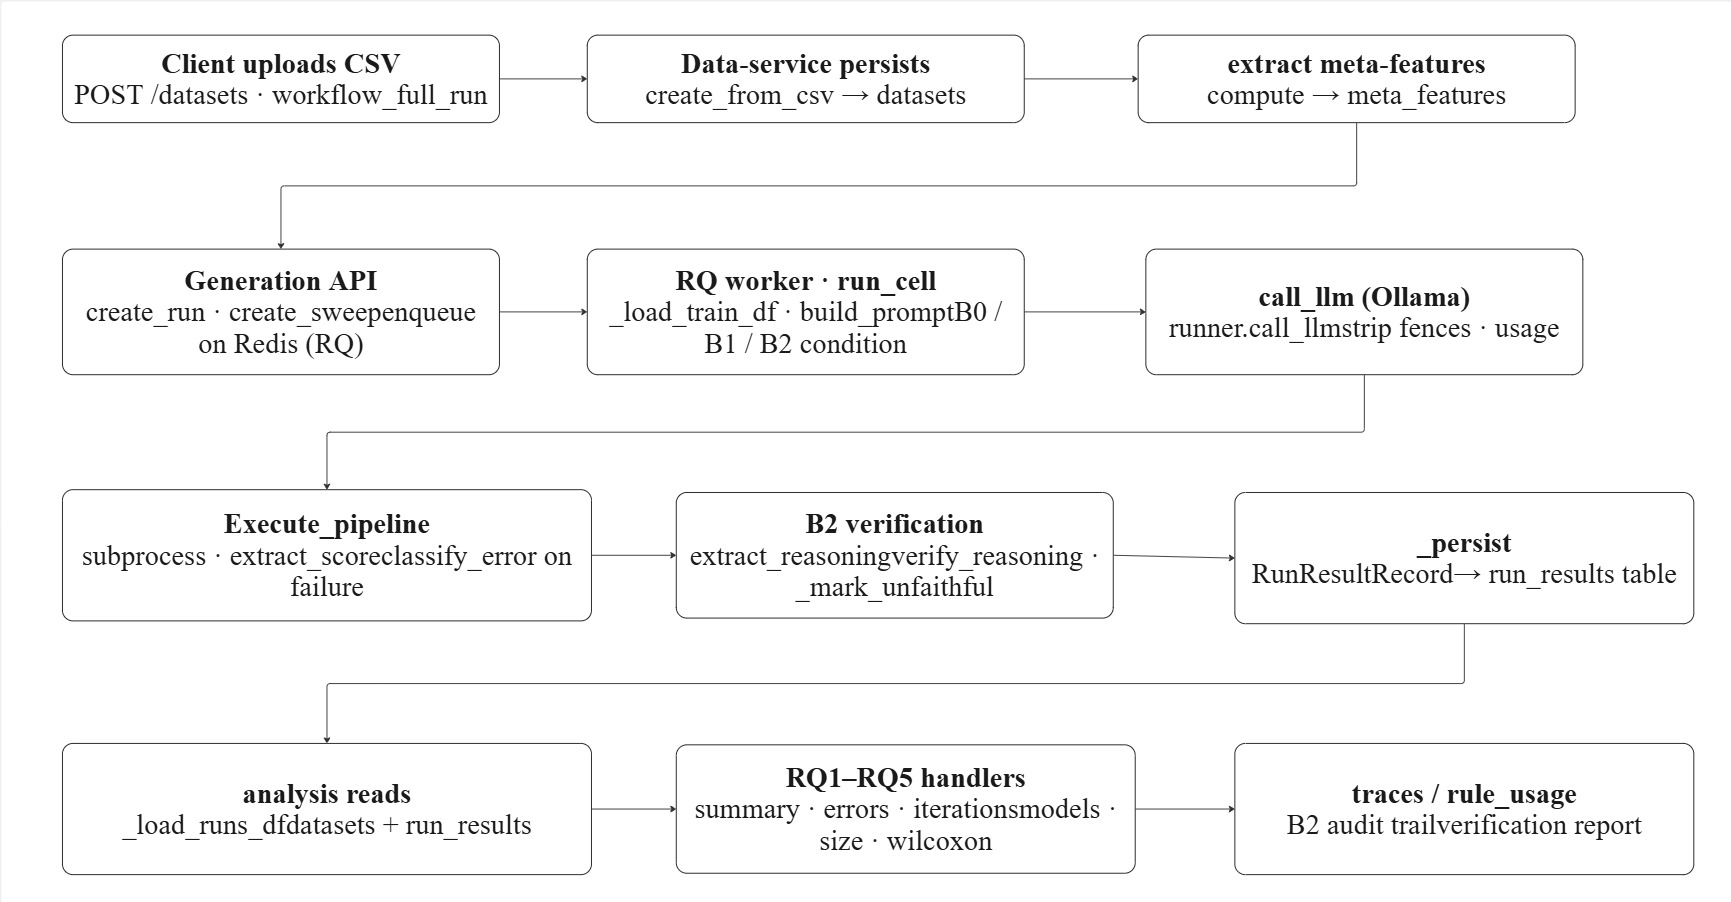
\includegraphics[width=0.84\textwidth]{figures/project_figures/architecture.png}
        \caption{Runtime flow of a single run: upload and meta--feature
        extraction, sweep enqueue, the \texttt{run\_cell} worker (prompt
        build, \texttt{call\_llm}, bounded--subprocess execution, B2
        verification), persistence to \texttt{run\_results}, and the
        read--only RQ1--RQ5 analysis.}
        \label{fig:architecture-flow}
    \end{subfigure}

    \vspace{0.3cm}

    \begin{subfigure}{\textwidth}
        \centering
        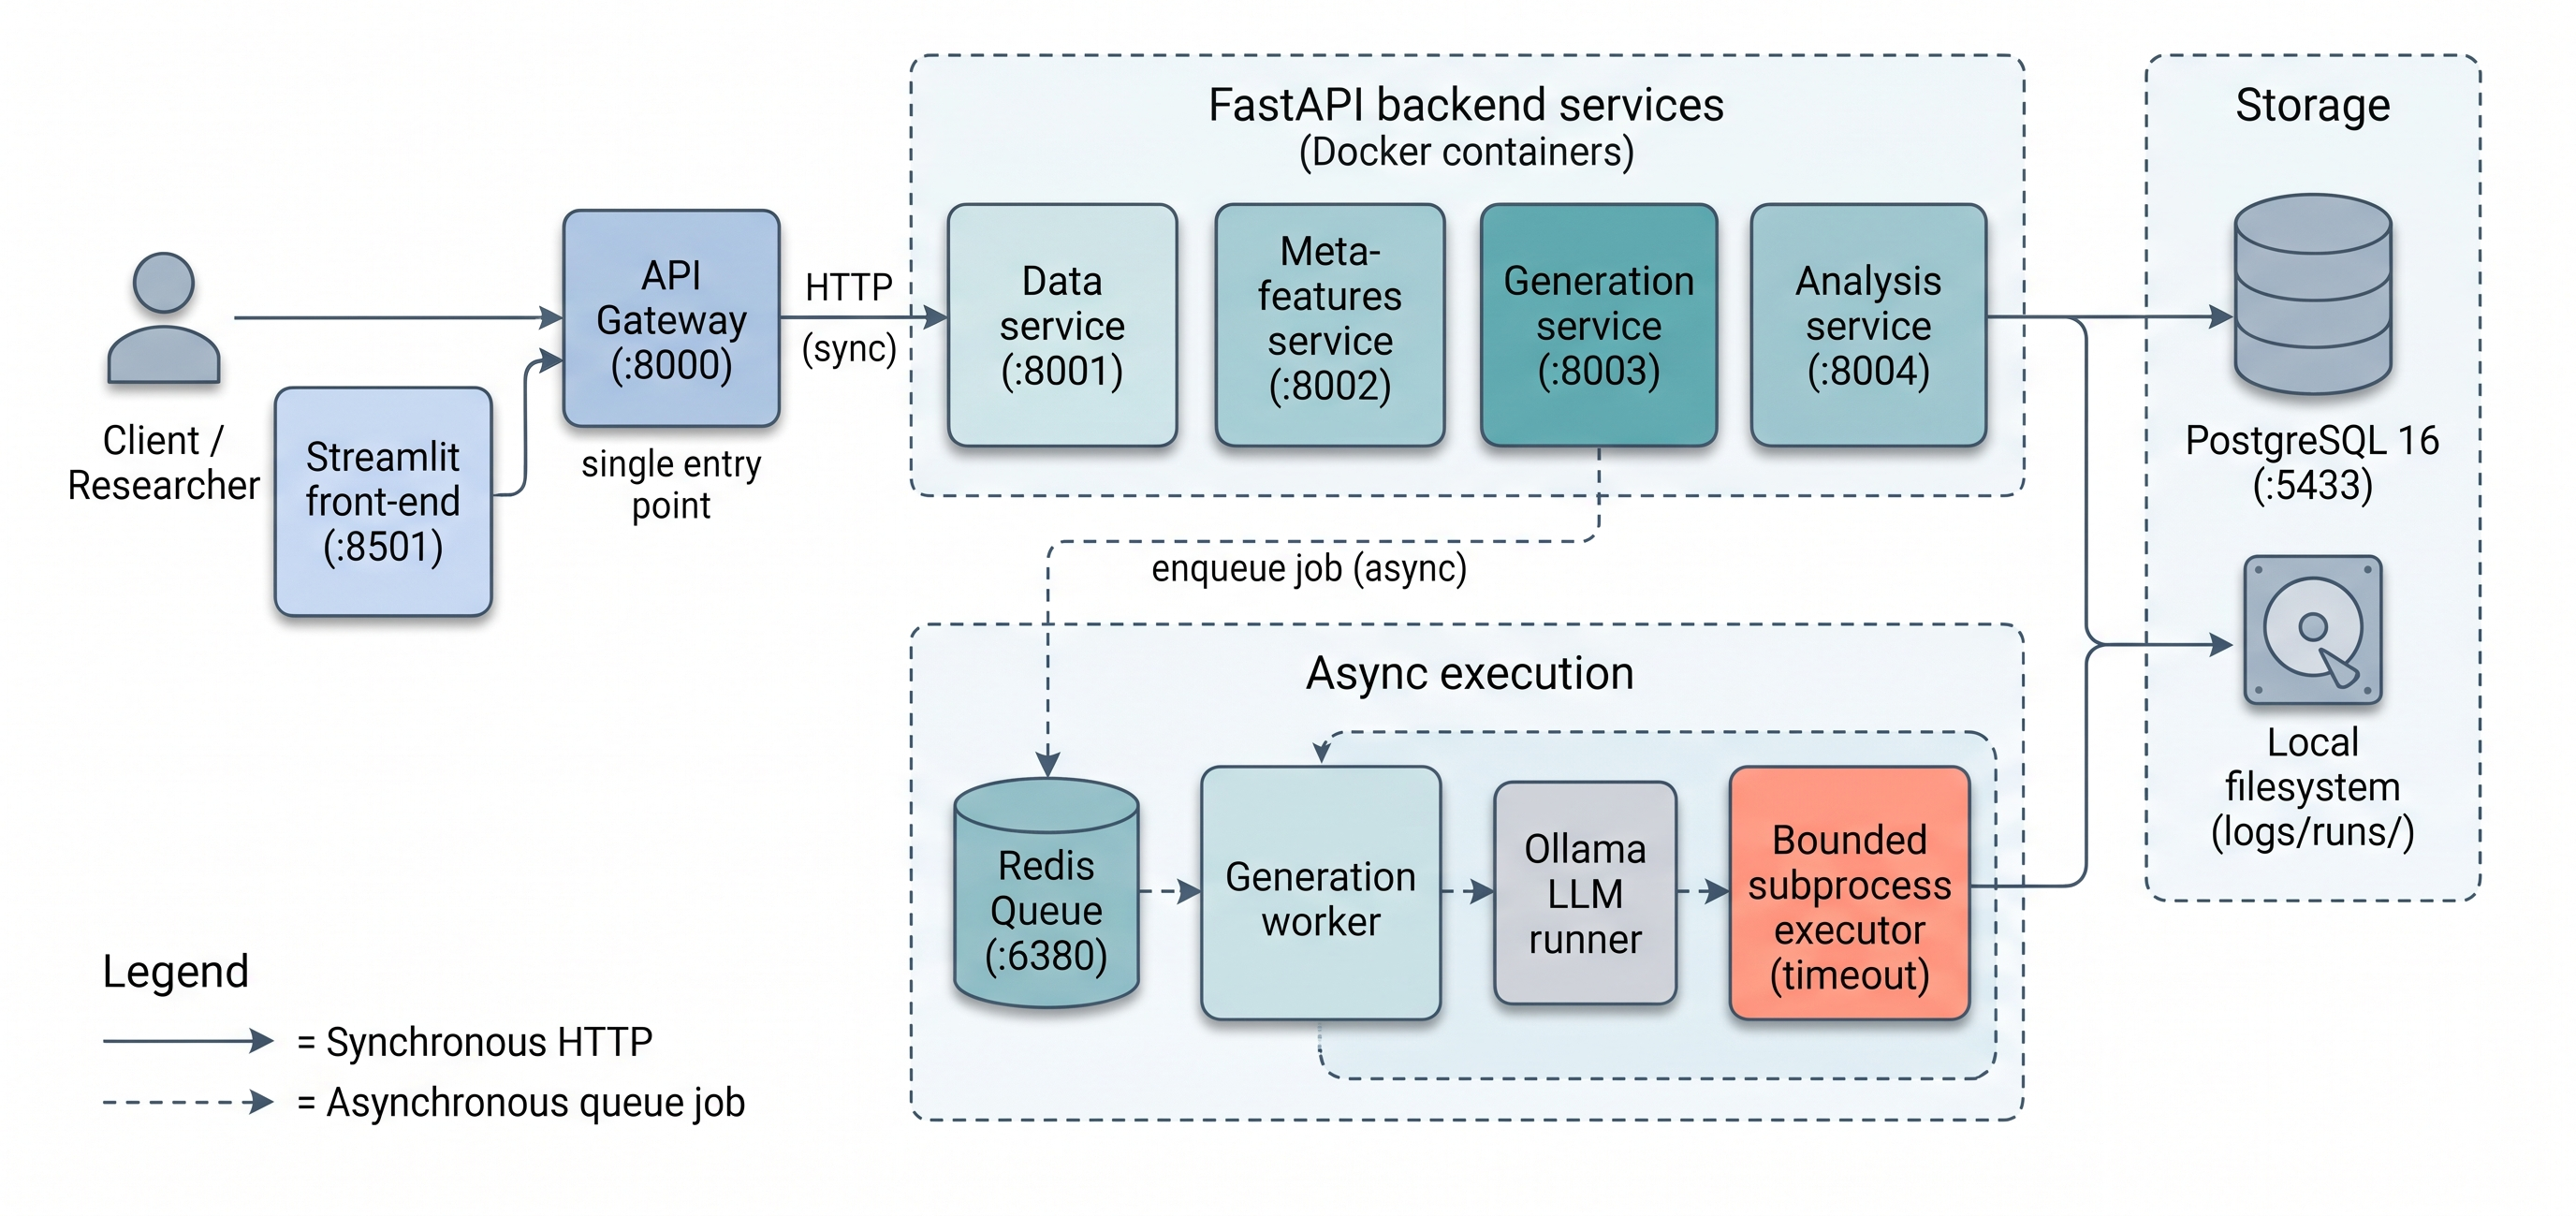
\includegraphics[width=0.84\textwidth]{figures/project_figures/BB_fig_4.1.2.png}
        \caption{Component and deployment view: the Streamlit front--end
        and clients reach the five FastAPI services through the gateway
        (synchronous HTTP); the generation service enqueues jobs on Redis
        for the worker, which drives the Ollama runner and the bounded
        subprocess executor (asynchronous); PostgreSQL and the local
        filesystem hold the results and artefacts. MinIO object storage is
        integrated in the code but was disabled for the reported runs.}
        \label{fig:architecture-components}
    \end{subfigure}
    \caption{System architecture: (a) the runtime flow of one run, and
    (b) the deployed components and their connections.}
    \label{fig:architecture}
\end{figure}

\subsection{Ingestion and Generation Tier}

The ingestion and generation tier exposes HTTP interfaces backed by
\textbf{FastAPI} services (served by \texttt{uvicorn}). A client
uploads a CSV via \texttt{POST /datasets} on the data service and
triggers a full workflow via the gateway. The data service persists
the dataset into the \texttt{datasets} table; the meta--features
service computes and caches the dataset's meta--feature profile into
the \texttt{meta\_features} table, keyed one--to--one by dataset. The
generation service then records a \texttt{sweep\_jobs} row and
enqueues one job per cell on the \textbf{Redis Queue (RQ)}. Note that
``RQ'' here denotes the Redis Queue job runner; the research
questions of this project are written \textbf{RQ1--RQ5} and are a
separate concept.

\subsection{Run and Verification Tier}

The run and verification tier is driven by a \textbf{Redis Queue (RQ)
worker} that executes the \texttt{run\_cell} task. The worker loads
the training dataframe, builds the generation prompt for one of the
three prompt conditions (\texttt{B0}, \texttt{B1}, \texttt{B2}) and
calls the configurable LLM runner (reached through
\texttt{call\_llm\_with\_usage}; the reported runs used hosted Ollama
cloud models), recording token usage.

The emitted pipeline is executed inside a bounded Python subprocess
(a separate process under a wall--clock timeout --- not container-level
isolation) that captures stdout and stderr, extracts the achieved score,
classifies failures into one of thirteen error categories and
preserves failed outcomes. For \texttt{B2} runs a verification stage
follows: the \textbf{implemented verifier} parses the reasoning trace
and, for each cited decision, checks that the named action appears in
the generated code's AST and that the cited statistic matches the
real meta--feature, yielding a boolean \texttt{faithful} verdict that
is persisted. The richer three--valued verdict with mismatch category
and source span specified in Chapter~\ref{ch:method} is the proposed
design; it is not produced by the current tier (see
Chapter~\ref{ch:impl}).

\subsection{Analysis Tier}

The analysis tier persists one \texttt{RunResultRecord} per cell into
the \texttt{run\_results} table. A set of RQ1--RQ5 handlers reads
\texttt{load\_runs}, \texttt{df}\_\texttt{datasets} and \texttt{run\_
results} and produces summaries, error counts, iteration models,
size versus wall--clock curves and the verification report that
answers the research questions. B2 audit trails are retained so that
any aggregate claim can be traced back to the individual verifier
decisions that produced it.

\section{System Workflow}

A single workflow proceeds along the three rows of
Fig.~\ref{fig:architecture-flow} as follows:

\begin{enumerate}
    \item \textbf{Request.} The client calls \texttt{POST
    /datasets} with a CSV and \texttt{POST /workflow\_full\_run}
    with the task specification. The data service persists the file
    and enqueues meta--feature extraction.
    \item \textbf{Sweep creation.} The generation service records a
    \texttt{sweep\_jobs} row and enqueues one job per cell on the
    Redis Queue.
    \item \textbf{Reasoning + code generation.} The RQ (Redis Queue)
    worker loads the training frame, selects the prompt condition
    (B0/B1/B2), calls the LLM runner and receives the generated
    pipeline code (and, under B2, a reasoning trace).
    \item \textbf{Execution.} \texttt{Execute\_pipeline} runs the
    code in a bounded subprocess, times out on hangs, and extracts the
    achieved score.
    \item \textbf{Verification (B2).} The implemented verifier checks
    each decision in the reasoning trace for action presence and
    meta--feature value grounding and records a boolean faithfulness
    verdict; the full RIR/PIR per--claim verdicts of
    Chapter~\ref{ch:method} are the proposed extension.
    \item \textbf{Persistence.} \texttt{\_persist} writes the run
    record (plan, code, trace, score, verdicts) to
    \texttt{run\_results}.
    \item \textbf{Analysis.} The RQ handlers aggregate the stored
    records into the summary, error, iteration, model--class, size
    and wildcard tables, and the trace/rule--usage report.
\end{enumerate}

\section{Use Case Diagram}

The three principal use cases are:

\begin{itemize}
    \item \emph{Submit workflow} --- a researcher uploads a dataset
    and a task specification, selects which research questions to
    exercise, and starts a sweep.
    \item \emph{Audit a run} --- a researcher opens a single run,
    inspects its code, execution trace and (for \texttt{B2}) the
    faithfulness verdict together with the reasons recorded for any
    failed check.
    \item \emph{Reproduce an analysis} --- a researcher regenerates
    the aggregate tables for RQ1--RQ5 from the stored run records,
    without re--running the LLM.
\end{itemize}

\begin{figure}[H]
    \centering
    \miroplaceholder[0.8\textwidth]{figures/project_figures/usecase.png}{%
    Use--case diagram with the actor ``Researcher'' and the three use
    cases: \emph{Submit workflow} (upload dataset + task, start a
    sweep), \emph{Audit a run} (inspect one run's plan, code, trace
    and faithfulness verdict), and \emph{Reproduce an analysis}
    (regenerate RQ1--RQ5 tables from stored rows without re--calling
    the LLM).}
    \caption{Principal use cases of the system.}
    \label{fig:usecase}
\end{figure}

\section{Data Flow}

Data flows through the system as follows:

\begin{itemize}
    \item CSV uploads enter the data service and are indexed by a
    dataset identifier. Meta--features derived from the dataset are
    stored alongside it.
    \item For each cell in a sweep, the RQ worker reads the training
    dataframe and composes a prompt that includes the dataset
    reference, the task type, and the RQ--specific instructions.
    \item The LLM returns a single, self--contained Python script,
    retained verbatim. Under \texttt{B2} the script, when run, also
    prints a structured reasoning trace (a small JSON object of
    decisions) that is captured from its output. The full PIR of
    Chapter~\ref{ch:method} is proposed and is not built here; the
    implemented check parses the code only into the set of names it
    references.
    \item The subprocess run returns a trace object with stdout, stderr,
    the extracted score (or an error classification) and timing
    data.
    \item For \texttt{B2}, the verifier returns a report whose fields
    are the number of decisions, the number found faithful, a single
    boolean \texttt{faithful} flag, and a per--decision list recording
    the step, the cited action, whether that action is present in the
    code, whether the cited value matched, and human--readable reasons
    for any failure. The richer records with mismatch category,
    severity and source span belong to the proposed design. These
    fields join the code, trace and score into a single
    \texttt{RunResultRecord}.
    \item The analysis handlers consume \texttt{RunResultRecord}s
    only; no handler reaches back into the live LLM, so analyses are
    repeatable from storage.
\end{itemize}

\section{Database Design}

The system of record is \textbf{PostgreSQL~16}, accessed through
SQLAlchemy ORM models. The schema has \emph{four} tables, defined so
that every aggregate report can be rebuilt from raw rows --- the
analysis layer only reads, and never writes derived values back.
Figure~\ref{fig:er} gives the entity--relationship overview and
Figures~\ref{fig:schema-dataset}--\ref{fig:schema-sweep} show the
actual ORM definitions.

\begin{itemize}
    \item \textbf{datasets} --- one row per registered dataset:
    \texttt{id}, \texttt{name}, \texttt{source}
    (\texttt{openml}/\texttt{custom}), \texttt{openml\_id},
    \texttt{target\_col}, \texttt{task\_type}, \texttt{train\_path},
    \texttt{test\_path}, \texttt{n\_rows}, \texttt{n\_cols},
    \texttt{created\_at}.
    \item \textbf{meta\_features} --- one row per dataset (enforced by
    a \texttt{UniqueConstraint} on \texttt{dataset\_id}): the full
    meta--feature profile as a \texttt{JSON} \texttt{features} column,
    plus \texttt{computed\_at}. This is the cache that the B2 prompt
    reads.
    \item \textbf{run\_results} --- one row per executed cell:
    \texttt{dataset\_id}, \texttt{condition}
    (\texttt{B0}/\texttt{B1}/\texttt{B2}), \texttt{llm\_backend},
    \texttt{seed}, \texttt{success}, \texttt{test\_score},
    \texttt{error\_category}, \texttt{iterations\_used},
    \texttt{runtime\_seconds}, \texttt{generated\_code\_path},
    \texttt{prompt\_tokens}, \texttt{completion\_tokens}, and ---
    for B2 only --- the \texttt{reasoning\_trace} and
    \texttt{verification\_report} as \texttt{JSON}.
    \item \textbf{sweep\_jobs} --- one row per enqueued sweep:
    \texttt{rq\_job\_id}, \texttt{status}, the cross--product
    \texttt{params} (\texttt{JSON}), and \texttt{total\_cells} /
    \texttt{completed\_cells} / \texttt{failed\_cells} progress
    counters.
\end{itemize}

Large artefacts (generated code, long traces) are written to the local
filesystem under \texttt{logs/runs/}, with a path reference kept in the
row. The stack also integrates \textbf{MinIO} object storage for these
artefacts, but MinIO was disabled in the evaluated deployment (its
images are no longer publicly pullable), so the reported runs used the
filesystem. Writes are idempotent: re--running a cell refreshes its row
rather than creating duplicates.

\begin{figure}[H]
    \centering
    \miroplaceholder{figures/project_figures/er_diagram.png}{%
    Entity--relationship diagram of the four tables ---
    \texttt{datasets} (1)\,$\rightarrow$\,(1) \texttt{meta\_features},
    \texttt{datasets} (1)\,$\rightarrow$\,(many) \texttt{run\_results},
    and the independent \texttt{sweep\_jobs} queue table --- showing
    primary keys, the \texttt{dataset\_id} foreign keys and the JSON
    columns.}
    \caption{Entity--relationship diagram of the PostgreSQL schema.}
    \label{fig:er}
\end{figure}

\begin{figure}[H]
    \centering
    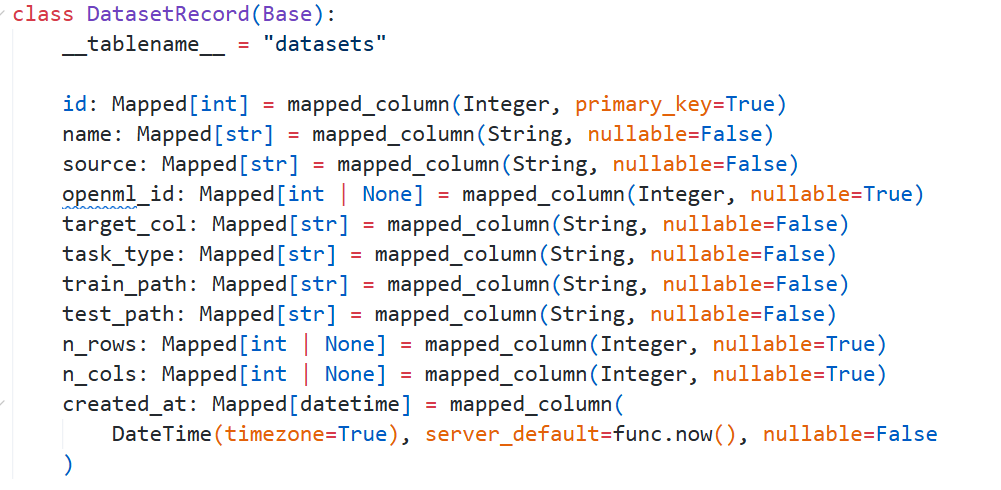
\includegraphics[width=0.92\textwidth]{figures/project_figures/screenshots/DatasetRecord.png}
    \caption{ORM model for the \texttt{datasets} table.}
    \label{fig:schema-dataset}
\end{figure}

\begin{figure}[H]
    \centering
    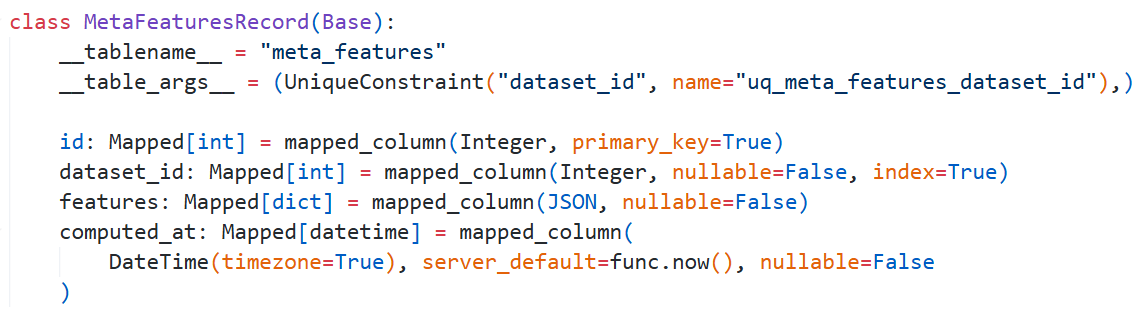
\includegraphics[width=0.92\textwidth]{figures/project_figures/screenshots/MetaFeatures_Schema.png}
    \caption{ORM model for the \texttt{meta\_features} table; the
    \texttt{UniqueConstraint} enforces one profile per dataset.}
    \label{fig:schema-meta}
\end{figure}

\begin{figure}[H]
    \centering
    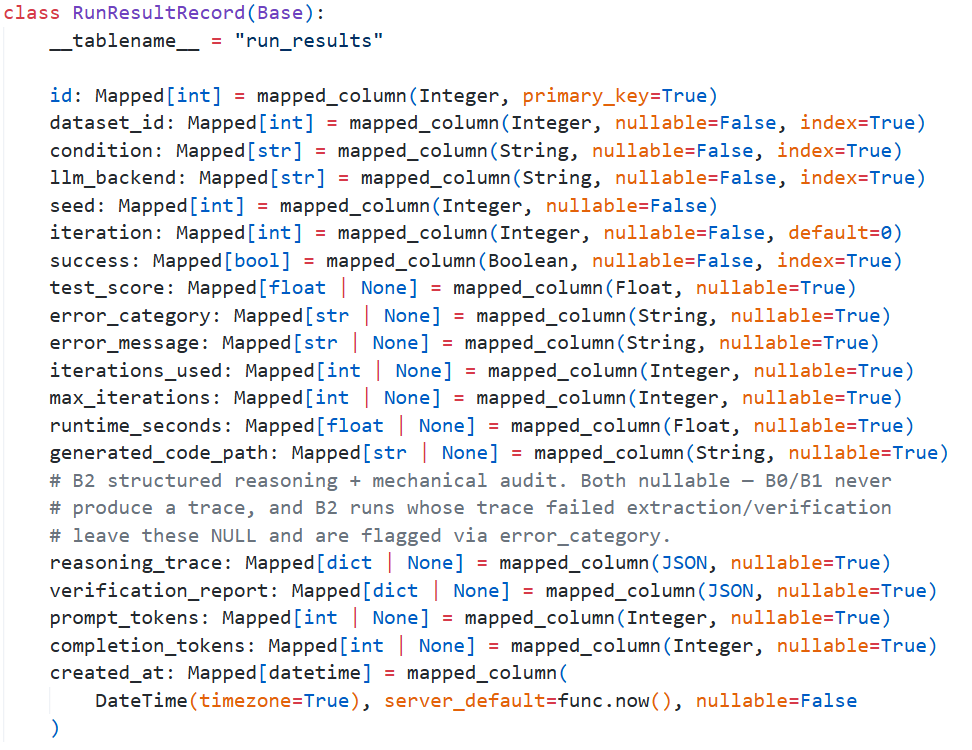
\includegraphics[width=0.92\textwidth]{figures/project_figures/screenshots/RunResultRecord.png}
    \caption{ORM model for the \texttt{run\_results} table; note the
    nullable B2--only \texttt{reasoning\_trace} and
    \texttt{verification\_report} JSON columns and the token counters.}
    \label{fig:schema-run}
\end{figure}

\begin{figure}[H]
    \centering
    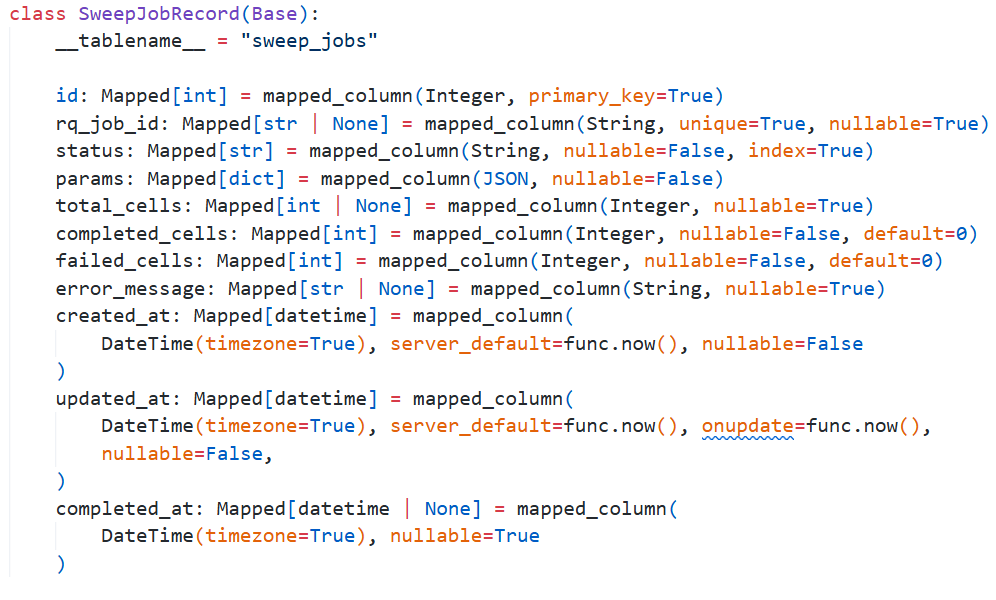
\includegraphics[width=0.92\textwidth]{figures/project_figures/screenshots/SweepJobRecord.png}
    \caption{ORM model for the \texttt{sweep\_jobs} table.}
    \label{fig:schema-sweep}
\end{figure}

\section{Module Description}

The system decomposes into eight modules.

\begin{enumerate}
    \item \textbf{Data Service.} Persists uploaded CSVs, extracts
    and stores meta--features, and exposes \texttt{create\_from\_csv}.
    \item \textbf{Generation API.} Orchestrates \texttt{create\_run}
    and the per--RQ sweep creation on Redis.
    \item \textbf{Prompt Builder.} Constructs the plan--emission and
    code--emission prompts for prompt classes \texttt{B0},
    \texttt{B1}, \texttt{B2} and conditional variants.
    \item \textbf{LLM Runner.} Wraps the configurable LLM backend
    (the reported runs used Ollama) as \texttt{runner.call\_llm} with
    explicit input/output fences and usage accounting.
    \item \textbf{Executor.} The \texttt{Execute\_pipeline} bounded
    subprocess executor that runs the generated code, extracts the
    score, classifies errors on failure and times out hangs.
    \item \textbf{Verifier.} The B2 module that checks, for each cited
    decision, action presence in the code and meta--feature value
    grounding, recording a boolean faithfulness verdict. Lowering the
    plan into the RIR and the code into the PIR to emit the per--claim
    verdicts of Chapter~\ref{ch:method} is the proposed extension and
    is not implemented in this project.
    \item \textbf{Persistence Layer.} \texttt{\_persist} writes the
    \texttt{RunResultRecord} and keeps the audit trail required for
    reproducibility.
    \item \textbf{Analysis Handlers.} RQ1--RQ5 handlers that render
    the summary, error, iteration, model, size and wildcard tables,
    together with the B2 audit/verification report.
\end{enumerate}

\chapter{Implementation}
\label{ch:impl}

This chapter reports what has actually been \emph{built and run} on
the project's \texttt{main} branch, and separates it cleanly from the
parts of Chapter~\ref{ch:method} that remain designed but unbuilt. It
is the honesty anchor of the report: the empirical results of
Chapter~\ref{ch:results} are produced only by the implemented
components described here.

\section{Implementation Status}

Table~\ref{tab:impl-status} classifies each component as
\emph{implemented} (exists and runs on \texttt{main}),
\emph{implemented (prototype)} (a first, deliberately narrow version),
or \emph{proposed} (specified in Chapter~\ref{ch:method}, not yet
coded).

\begin{table}[H]
\centering
\caption{Implementation status of each system component.}
\label{tab:impl-status}
\small
\renewcommand{\arraystretch}{1.25}
\begin{tabular}{p{8.2cm} p{4.6cm}}
\toprule
\textbf{Component} & \textbf{Status} \\
\midrule
Five FastAPI services (data, meta--features, generation, analysis,
gateway) plus two front--ends (Streamlit, Next.js) & Implemented \\
Redis Queue worker + sweep orchestration (\texttt{sweep\_jobs}) &
Implemented \\
Three prompt conditions B0 / B1 / B2 & Implemented \\
Ollama LLM runner (three cloud backends) & Implemented \\
Sandboxed subprocess executor + 13--category error taxonomy &
Implemented \\
Meta--feature extraction (four families) & Implemented \\
PostgreSQL + MinIO persistence; JSON trace / report sidecars &
Implemented \\
RQ1--RQ5 analysis endpoints, \texttt{/analysis/traces},
\texttt{/analysis/rule-usage} & Implemented \\
Faithfulness verifier: action--presence + value--grounding, boolean
verdict & Implemented (prototype) \\
AST--based Program IR; existence / parameter / ordering / column
checks; three--valued claim + four--valued pipeline verdicts; partial
taxonomy; verifier CLI & Implemented (prototype;
\texttt{feat/rir-pir-verifier}) \\
Graph--based (multigraph) Program IR; set--valued mapper; full
mismatch taxonomy as emitted categories; verification dashboard &
Proposed \\
Independent pre--code reasoning (\texttt{B2R} mode) & Proposed \\
\bottomrule
\end{tabular}
\end{table}

\section{Development Environment}

\begin{itemize}
    \item \textbf{Language.} Python 3.10+.
    \item \textbf{Services.} \texttt{FastAPI} with \texttt{uvicorn};
    each service is a separate git repository with its own
    \texttt{Dockerfile}. The \texttt{automl-infra} repository holds
    the Docker Compose definition and the SQL migrations.
    \item \textbf{ML libraries.} \texttt{scikit--learn},
    \texttt{pandas}, \texttt{numpy}, \texttt{scipy}.
    \item \textbf{Program analysis.} The implemented verifier uses the
    standard--library \texttt{ast} module only. The
    \texttt{networkx}/\texttt{libcst} graph layer of
    Chapter~\ref{ch:method} is \emph{not} a current dependency.
    \item \textbf{LLM runner.} \texttt{Ollama}, wrapped by
    \texttt{call\_llm\_with\_usage} so that the backend can be swapped
    and token usage recorded. The evaluated backends are
    \texttt{gpt-oss:120b-cloud}, \texttt{gemma4:31b-cloud} and
    \texttt{nemotron-3-nano:30b-cloud}.
    \item \textbf{Storage.} \textbf{PostgreSQL~16} is the system of
    record; \textbf{MinIO} holds large artefacts; \textbf{Redis~7}
    backs the job queue.
    \item \textbf{Tooling.} Per--repository \texttt{git}, \texttt{pytest}
    for unit tests, and this \LaTeX{} report.
\end{itemize}

\section{Implemented Services}

The stack is seven small services behind a gateway, each with an HTTP
API and its own container (Table~\ref{tab:services}).

\begin{table}[H]
\centering
\caption{The seven services and their ports.}
\label{tab:services}
\small
\renewcommand{\arraystretch}{1.2}
\begin{tabular}{p{4.2cm} p{1.4cm} p{7cm}}
\toprule
\textbf{Service} & \textbf{Port} & \textbf{Responsibility} \\
\midrule
\texttt{automl-data-service} & 8001 & Register a CSV or fetch an
OpenML dataset; persist rows + metadata. \\
\texttt{automl-metafeatures-service} & 8002 & Compute / cache the
meta--feature profile for a dataset. \\
\texttt{automl-generation-service} & 8003 & Enqueue code--generation
jobs on Redis; a worker runs, executes and verifies them. \\
\texttt{automl-analysis-service} & 8004 & Read--only analytics:
success rates, iterations, error mix, significance tests, trace and
rule--usage reports. \\
\texttt{automl-gateway} & 8000 & Single entry point; composes
\texttt{upload-and-extract} and \texttt{full-run} workflows. \\
\texttt{automl-frontend} / \texttt{-openui} & --- & Streamlit and
Next.js front--ends for browsing datasets and runs. \\
\bottomrule
\end{tabular}
\end{table}

Shared logic lives in the \texttt{automl-reusables} library (imported
by every service): the meta--feature extractors, the prompt
conditions, the executor, the error taxonomy and the verifier.

\subsection{Data Service}

The data service accepts a CSV at \texttt{POST /datasets} or fetches
an OpenML dataset by id, performs a deterministic stratified
train/test split, writes the CSVs to a dataset--identified folder and
persists a \texttt{datasets} row. It never forwards raw rows to the
LLM; only derived descriptors are exposed downstream
(Fig.~\ref{fig:data-svc}).

\begin{figure}[H]
    \centering
    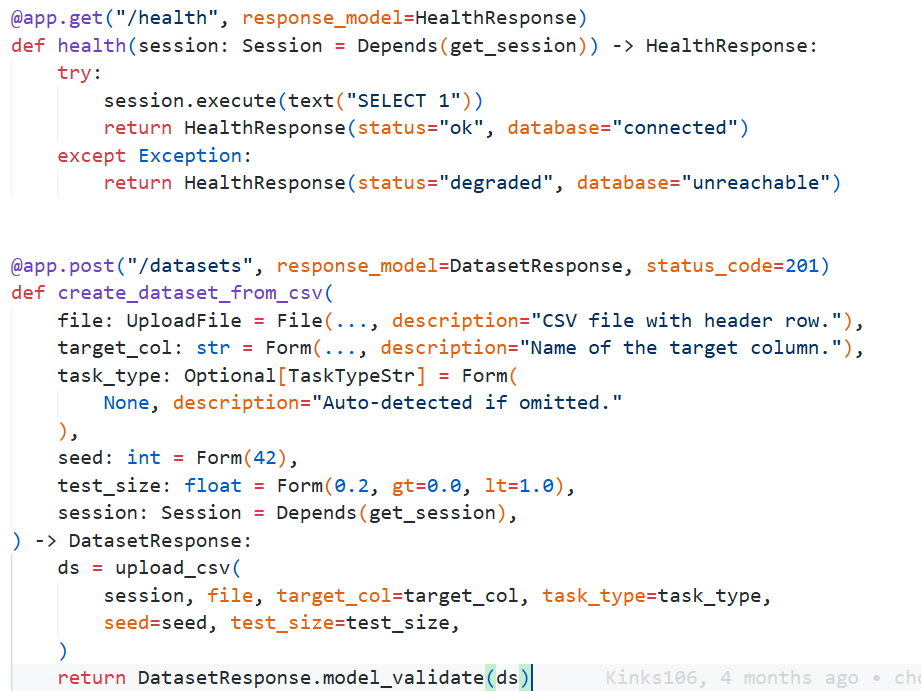
\includegraphics[width=0.9\textwidth]{figures/project_figures/screenshots/data_generation_service_1.png}
    \caption{Data--service ingestion path (dataset registration and
    split).}
    \label{fig:data-svc}
\end{figure}

\subsection{Meta-Feature Service}

For each dataset the service computes one JSON meta--feature object
with four families --- \emph{simple} (counts, missingness,
cardinality, class balance), \emph{distributional} (skewness,
kurtosis, outlier ratio), \emph{information} (mutual information,
pairwise correlation, target entropy) and \emph{landmarking} (decision
stump, linear/NB and 1--NN reference scores) --- and caches it in the
\texttt{meta\_features} table. Column typing is handled by small,
deterministic helpers (Fig.~\ref{fig:mf-helpers}).

\begin{figure}[H]
    \centering
    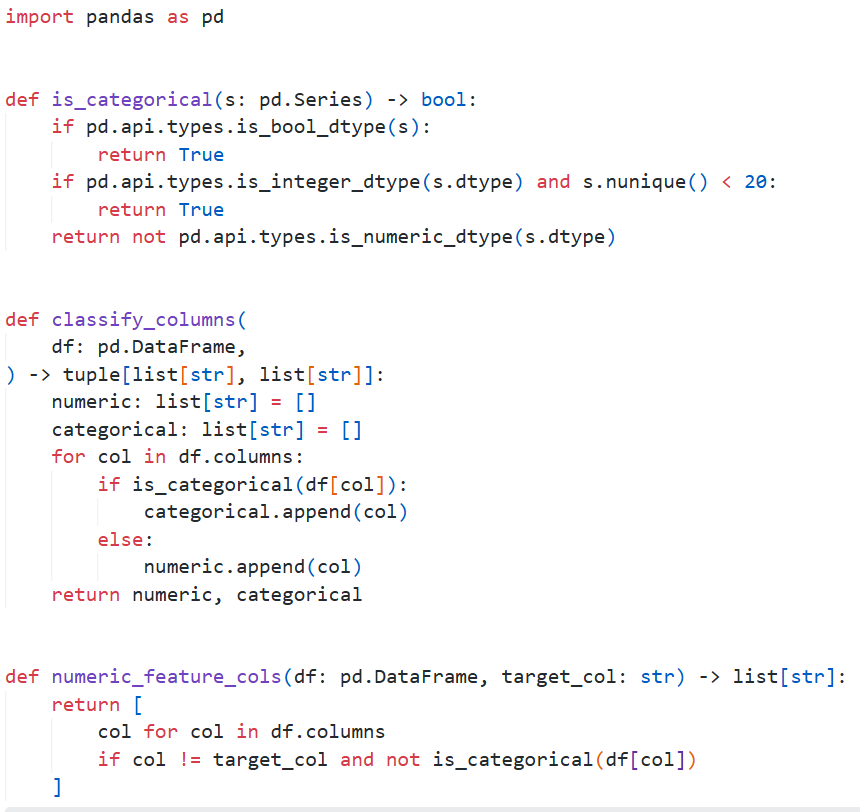
\includegraphics[width=0.78\textwidth]{figures/project_figures/screenshots/metaFetaures_helpers.png}
    \caption{Meta--feature helpers: a column is categorical if boolean,
    low--cardinality integer, or non--numeric.}
    \label{fig:mf-helpers}
\end{figure}

\subsection{Prompt Conditions: B0, B1, B2}

The three conditions are the experiment's independent variable and
differ \emph{only} in prompt content; the code that executes, scores
and persists their output is identical.

\begin{itemize}
    \item \textbf{B0 (naive).} Task description only, plus the hard
    requirement that every class/function be explicitly imported.
    \item \textbf{B1 (schema).} B0 plus a dataset--schema section:
    row/column counts, task type, target column, column dtypes and the
    first three rows.
    \item \textbf{B2 (meta--feature--guided).} B1 plus the full
    meta--feature JSON, fourteen numbered decision rules, a
    cite--your--reasoning instruction, and a \emph{mandatory,
    machine--verified} structured reasoning trace that the generated
    script must print at runtime (Fig.~\ref{fig:b2-prompt}).
\end{itemize}

\begin{figure}[H]
    \centering
    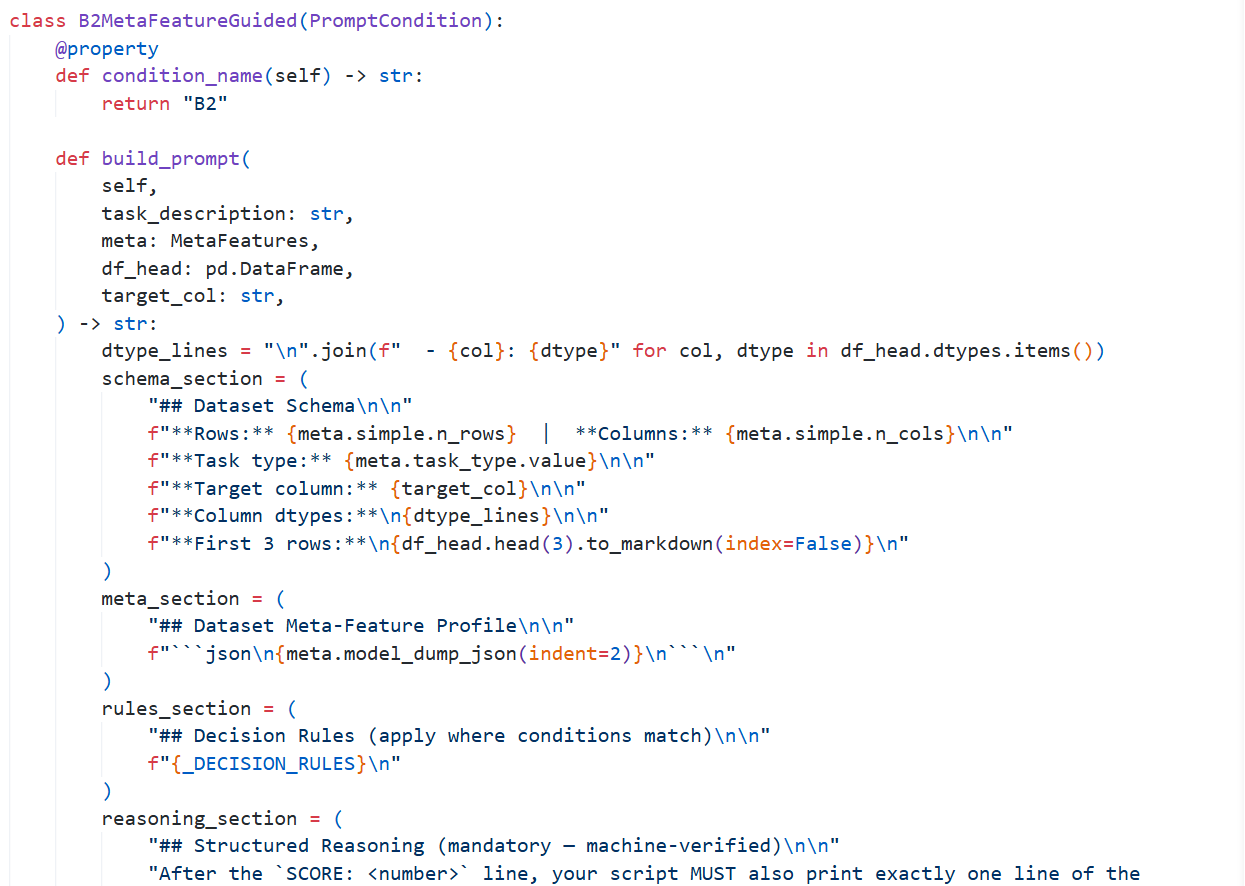
\includegraphics[width=0.95\textwidth]{figures/project_figures/screenshots/b2_metafeatures_1.png}
    \caption{The B2 prompt builder assembling the schema,
    meta--feature profile, decision rules and mandatory
    reasoning--trace sections.}
    \label{fig:b2-prompt}
\end{figure}

A consequence worth stating plainly: because the B2 reasoning trace is
printed by the \emph{generated code at runtime}, it is a post--hoc
self--report derived from the code, not a plan captured independently
\emph{before} the code. Capturing an independent pre--code plan (the
\texttt{B2R} mode of Chapter~\ref{ch:method}) is designed but not yet
wired, and is the single most important limitation of the current
verifier.

\subsection{Generation Service and RQ Worker}

The generation service records a \texttt{sweep\_jobs} row and enqueues
one Redis Queue job per cell; a worker container pulls each job, runs
\texttt{jobs.run\_cell}, and retries up to \texttt{max\_iterations}
times, feeding the classified error back to the LLM as a hint on each
retry (Fig.~\ref{fig:gen-svc}).

\begin{figure}[H]
    \centering
    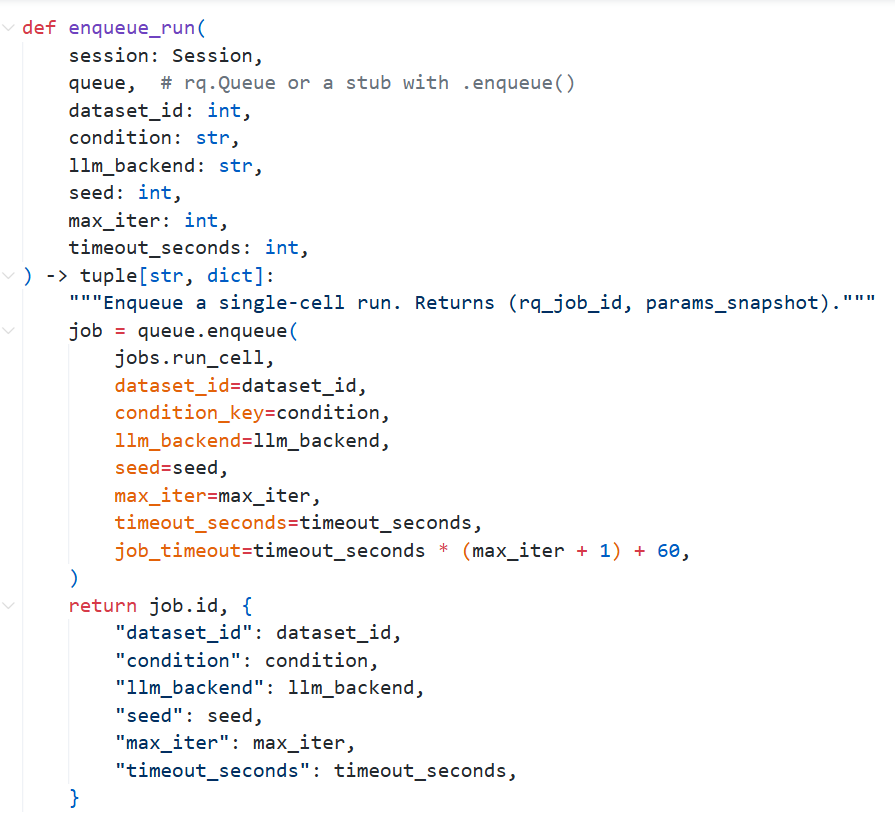
\includegraphics[width=0.82\textwidth]{figures/project_figures/screenshots/generation_service_py.png}
    \caption{Enqueuing one sweep cell as a Redis Queue job; the job
    runs \texttt{jobs.run\_cell} on a worker.}
    \label{fig:gen-svc}
\end{figure}

\subsection{Sandboxed Executor and Error Taxonomy}

Generated code is written to a temporary file and run in a fresh
Python subprocess with a per--attempt wall--clock budget; stdout,
stderr and the return code are captured and the printed
\texttt{SCORE:} line is parsed. Execution failures are classified into
the thirteen--category \texttt{ErrorCategory} taxonomy: a
priority--ordered, \texttt{stderr}--based classifier assigns the
code--failure categories (\texttt{syntax\_error}, \texttt{import\_error},
\texttt{api\_hallucination}, \texttt{shape\_mismatch},
\texttt{type\_error}, \texttt{missing\_name}, \texttt{timeout},
\texttt{resource\_limit} and others), the leakage guard assigns
\texttt{suspicious\_leakage}, and the B2 verifier assigns
\texttt{reasoning\_unfaithful}. Infrastructure--level failures (such as
a failed LLM call) are recorded under a separate \texttt{infrastructure}
label, so that LLM/prompt failures are never confused with
infrastructure failures (Fig.~\ref{fig:err-tax}).

\begin{figure}[H]
    \centering
    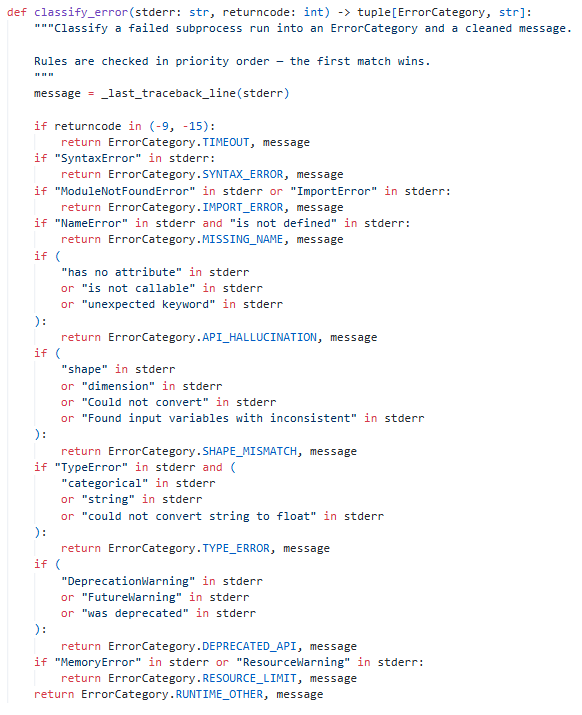
\includegraphics[width=0.66\textwidth]{figures/project_figures/screenshots/error_taxonomy.png}
    \caption{The rule--based execution--error classifier
    (\texttt{classify\_error}); the first matching rule wins.}
    \label{fig:err-tax}
\end{figure}

\subsection{Implemented Verifier (Prototype)}
\label{subsec:impl-verifier}

The implemented verifier (\texttt{execution/verification.py}) realises
a deliberately narrow subset of Chapter~\ref{ch:method}, and only for
B2 runs. For each decision in the reasoning trace it performs two
pure--Python checks:

\begin{enumerate}
    \item \textbf{Action presence.} Parse the generated code with
    \texttt{ast} into a set of referenced names (imports, called
    functions, attributes, bare identifiers). The decision passes if
    its cited \texttt{action} symbol is in that set --- catching a
    preprocessor the LLM \emph{claimed} but never used.
    \item \textbf{Value grounding.} Follow the decision's cited
    \texttt{meta\_feature} dotted path into the real meta--feature
    object and compare the LLM's cited \texttt{observed\_value} within
    a $10^{-3}$ tolerance --- catching a \emph{fabricated or
    misremembered} number.
\end{enumerate}

A run is \texttt{faithful} iff every decision passes both checks; an
unfaithful run is recorded with \texttt{error\_category =
reasoning\_unfaithful}. The current code treats an \emph{uncheckable}
value (no numeric path to compare) as not--contradicted; the proposed
three--valued verdict of Chapter~\ref{ch:method} would instead return
\textsc{unverifiable} here, and closing this gap is listed as future
work. This verifier is the mechanism behind the faithfulness result of
Chapter~\ref{ch:results} (Section~\ref{sec:rq5}).

\paragraph{RIR/PIR prototype (feature branch).} A larger prototype of
the Chapter~\ref{ch:method} verifier exists on the
\texttt{feat/rir-pir-verifier} branch (stdlib \texttt{ast} and
\texttt{dataclasses}, not merged into \texttt{main} and not wired into
the run tier). It lowers a plan into the RIR and the generated code
into an AST--based PIR, applies existence, parameter, column and
ordering rules to produce a three--valued per--claim verdict, and
aggregates these --- with criticality gating --- into a four--valued
pipeline verdict, exposed through a small command--line tool. It
realises the core of the proposed design short of the graph--based PIR
and the set--valued mapper, and has so far been exercised only on a
small set of hand--checked cases, not on the 270--run sweep.

\subsection{Persistence and Analysis}

Each cell is persisted as a \texttt{run\_results} row; the B2
\texttt{reasoning\_trace} and \texttt{verification\_report} are stored
as JSON columns and also written as \texttt{.trace.json} /
\texttt{.verification.json} sidecars to MinIO. The analysis service
exposes one read--only endpoint per research question plus
\texttt{/analysis/traces} and \texttt{/analysis/rule-usage}; because
it only reads persisted rows, every table in Chapter~\ref{ch:results}
can be regenerated without re--calling any LLM.

\section{Proposed Components (Designed, Not Yet Implemented)}

Beyond the \texttt{main} verifier, the prototype of
Section~\ref{subsec:impl-verifier} (branch
\texttt{feat/rir-pir-verifier}) already implements an AST--based
Program IR, existence / parameter / ordering / column checks,
three--valued per--claim and four--valued pipeline verdicts over a
partial taxonomy, and a standalone CLI; it is not merged into
\texttt{main}, not wired into the run tier, and not validated at the
scale of the 270--run study. The remaining parts of
Chapter~\ref{ch:method} are \emph{not} built anywhere and are not drawn
upon by the 270--run study of Chapter~\ref{ch:results}: the
graph--based (multigraph) Program IR; the set--valued
claim--to--witness mapper with learned ranking; the full mismatch
taxonomy as emitted categories; and a verification--result dashboard.
The independent pre--code reasoning capture (\texttt{B2R}) is likewise
designed but not wired.

\section{Algorithm: Implemented vs Proposed}

The implemented \texttt{main} verifier is the compact routine on the
left (presence and value grounding only); the routine on the right is
the proposed full verifier, most of which --- the RIR, the AST--based
PIR, the three--valued conjunction over presence, parameters and
ordering, and the aggregation --- is realised by the prototype of
Section~\ref{subsec:impl-verifier}, short of the graph PIR and the
set--valued mapper.

\begin{lstlisting}[language=Python,caption={Implemented: boolean faithfulness check (prototype v1).}]
def verify_reasoning(trace, code, meta):
    code_names = names_in_code(code)      # ast walk -> set[str]
    verdicts = []
    for d in trace.decisions:
        present = d.action in code_names          # presence
        value_ok = value_matches(d.observed_value,
                                 lookup(meta, d.meta_feature))  # grounding
        verdicts.append((present, value_ok))
    faithful = len(verdicts) > 0 and all(
        p and (v is not False) for p, v in verdicts)
    return VerificationReport(faithful=faithful, verdicts=verdicts)
\end{lstlisting}

\begin{lstlisting}[language=Python,caption={Proposed: full RIR--PIR claim verdicts (designed, Chapter~\ref{ch:method}).}]
def verify(plan, code):                   # PROPOSED
    rir = build_rir(plan)                  # atomic typed claims
    pir = build_pir(code)                  # attributed multigraph
    verdicts = []
    for r in rir:
        cands = mapper(r, pir)             # set-valued witness
        v = three_valued_and(presence(r, cands), semantics(r, cands),
                              parameters(r, cands), ordering(r, pir),
                              dependency(r, pir))
        verdicts.append(ClaimReport(r, cands, v, classify(r, cands, v)))
    return aggregate(verdicts)             # coverage, S_align, CMR, loc.
\end{lstlisting}

\section{Security and Privacy}

The verifier executes untrusted LLM--generated code, so the sandbox is
the main security concern. Mitigations: the subprocess runs with a
bounded wall--clock budget in a temporary working directory that is
discarded afterwards; a leakage guard flags any near--perfect score
(\texttt{>=0.995}) on a classification task for review; and raw
dataset rows are never sent to the LLM runner --- only meta--features
and column descriptors are. Static import pinning and a private--bound
API with a key are specified for deployment and are partially in place.

\section{Summary}

The implemented system is a running, seven--service FastAPI stack that
generates scikit--learn pipelines under three prompt conditions,
executes them in a sandbox, classifies failures, and --- for B2 ---
mechanically checks the reasoning trace for action presence and
value grounding, persisting everything to PostgreSQL and MinIO. The
full graph--based verifier of Chapter~\ref{ch:method} remains proposed.
The next chapter evaluates exactly what is implemented here on a real
270--cell experimental sweep.

\chapter{Results and Discussion}
\label{ch:results}

This chapter reports measured results from a real experimental run of
the implemented system (Chapter~\ref{ch:impl}). Every number is
traceable to the recorded run; no value is a placeholder or an
estimate. Where a research question requires the full verifier of
Chapter~\ref{ch:method}, which is not yet built, the question is
answered as far as the implemented main--branch verifier (presence and
value grounding) allows and the remainder is marked as future work.

\section{Experimental Setup}

The evaluation is a controlled \textbf{270--cell sweep}. The unit of
analysis is a cell --- a tuple
\[
(\text{dataset}, \text{condition}, \text{LLM backend}, \text{seed}),
\]
and the design is the full cross--product of \textbf{6 datasets
$\times$ 3 conditions $\times$ 3 backends $\times$ 5 seeds}. Each cell
produces one \texttt{run\_results} row.

\begin{itemize}
    \item \textbf{Conditions.} B0 (naive), B1 (schema), B2
    (meta--feature--guided), as implemented in
    Chapter~\ref{ch:impl}.
    \item \textbf{Backends.} \texttt{gpt-oss:120b-cloud},
    \texttt{gemma4:31b-cloud} and \texttt{nemotron-3-nano:30b-cloud},
    served through Ollama.
    \item \textbf{Seeds.} 3001--3005 (five), fixing the train/test
    split and generation seed so comparisons across conditions are
    paired on the same cell.
    \item \textbf{Metric.} All six datasets are binary
    classification; the score is \texttt{balanced\_accuracy} on a
    held--out test split (higher is better), chosen so that a
    majority--class predictor cannot score well.
    \item \textbf{Max iterations.} 3; a cell is a failure if no
    runnable, verified pipeline is produced within three attempts.
\end{itemize}

The run completed in 5\,h\,17\,m. A leakage guard (any
\texttt{balanced\_accuracy} $\geq 0.995$ on a classification task)
fired on \textbf{zero} cells. All artefacts (generated code, traces,
verification reports) are persisted, so the tables below can be
regenerated from storage without re--calling any LLM.

\begin{quote}
\textbf{Note on earlier data.} An initial mid--term snapshot
(2026--07) contained only six runs under a single condition and is
\emph{not} used here; it has been fully superseded by the 270--cell
sweep. A first sweep attempt was also discarded after a mid--run
reboot corrupted it; the reported run is the clean redo.
\end{quote}

\subsection{Datasets}

\begin{table}[H]
\centering
\caption{The six--dataset panel (all binary classification).}
\label{tab:datasets}
\small
\renewcommand{\arraystretch}{1.2}
\begin{tabular}{l r r l}
\toprule
\textbf{Dataset} & \textbf{Rows} & \textbf{Cols} & \textbf{Source} \\
\midrule
wdbc        & 569  & 31 & OpenML 1510 \\
breast-w    & 699  & 10 & OpenML 15 \\
diabetes    & 768  & 9  & OpenML 37 \\
Titanic     & 891  & 11 & curated \\
spambase    & 4601 & 58 & OpenML 44 \\
Telco churn & 7043 & 21 & curated (IBM) \\
\bottomrule
\end{tabular}
\end{table}

\section{Pipeline-Level Results}

Table~\ref{tab:percond} gives the headline per--condition result
collapsed over all datasets, backends and seeds (90 cells each).

\begin{table}[H]
\centering
\caption{Per--condition results over all 90 cells each. ``Mean score''
and ``Mean iters'' are over successful runs only.}
\label{tab:percond}
\renewcommand{\arraystretch}{1.3}
\begin{tabular}{l r r r r}
\toprule
\textbf{Condition} & \textbf{Success} & \textbf{Success \%} &
\textbf{Mean score} & \textbf{Mean iters} \\
\midrule
B0 (naive)        & 90/90 & 100.0\,\% & 0.8432 & 1.01 \\
B1 (schema)       & 90/90 & 100.0\,\% & 0.8468 & 1.06 \\
B2 (meta-feature) & 56/90 & \textbf{62.2\,\%} & 0.8549$^\ast$ & 1.41 \\
\bottomrule
\end{tabular}
\end{table}

\noindent$^\ast$ B2's marginally higher mean is \emph{survivorship
bias}: only the 56 cells it completes contribute, while its 34
failures (often the harder cells) are excluded. The paired test in
Section~\ref{sec:rq4} is the valid comparison.

The breakdown by backend (Table~\ref{tab:permodel}) shows the effect
is uniform and that B2 is far more expensive. B0 and B1 are perfectly
reliable across all three backends; B2 drops every backend and is
catastrophic for the smallest (nemotron--nano, 26.7\,\%), whose
run--away completion length (26k tokens) trips upstream limits.

\begin{table}[H]
\centering
\caption{Per--backend $\times$ condition: success, iterations
(averaged over all 30 cells, including failed attempts) and token
cost (averages).}
\label{tab:permodel}
\scriptsize
\renewcommand{\arraystretch}{1.25}
\begin{tabular}{l l r r r r r}
\toprule
\textbf{Backend} & \textbf{Cond} & \textbf{ok/30} & \textbf{succ\%} &
\textbf{iters} & \textbf{prompt tok} & \textbf{compl.\ tok} \\
\midrule
gemma4:31b-cloud          & B0 & 30 & 100.0 & 1.00 & 348  & 627 \\
gemma4:31b-cloud          & B1 & 30 & 100.0 & 1.00 & 1182 & 611 \\
gemma4:31b-cloud          & B2 & 24 & 80.0  & 1.87 & 9280 & 2506 \\
gpt-oss:120b-cloud        & B0 & 30 & 100.0 & 1.00 & 369  & 1338 \\
gpt-oss:120b-cloud        & B1 & 30 & 100.0 & 1.03 & 1170 & 1346 \\
gpt-oss:120b-cloud        & B2 & 24 & 80.0  & 1.70 & 6449 & 5330 \\
nemotron-3-nano:30b-cloud & B0 & 30 & 100.0 & 1.03 & 348  & 2112 \\
nemotron-3-nano:30b-cloud & B1 & 30 & 100.0 & 1.13 & 1433 & 2660 \\
nemotron-3-nano:30b-cloud & B2 & 8  & \textbf{26.7} & 1.33 & 7373 & \textbf{26244} \\
\bottomrule
\end{tabular}
\end{table}

\begin{figure}[H]
    \centering
    \miroplaceholder{figures/project_figures/fig_success_by_condition.png}{%
    Grouped bar chart of success rate (\%) by condition, one group per
    backend; B0 and B1 at 100\,\% and B2 at 80/80/27\,\%. A second
    panel can overlay mean prompt tokens to show B2's cost.}
    \caption{Success rate by condition and backend.}
    \label{fig:success}
\end{figure}

Table~\ref{tab:perdataset} reports mean test score per dataset and
condition. On every dataset the three conditions land within $\pm
0.02$ of each other; meta--features do not shift pipeline quality.

\begin{table}[H]
\centering
\caption{Mean \texttt{balanced\_accuracy} per dataset $\times$
condition (successful runs; ``ok'' = successes of 15).}
\label{tab:perdataset}
\scriptsize
\renewcommand{\arraystretch}{1.25}
\begin{tabular}{l r | r r | r r | r r}
\toprule
& & \multicolumn{2}{c|}{\textbf{B0}} & \multicolumn{2}{c|}{\textbf{B1}}
& \multicolumn{2}{c}{\textbf{B2}} \\
\textbf{Dataset} & \textbf{rows} & ok & score & ok & score & ok & score \\
\midrule
wdbc        & 569  & 15 & 0.9618 & 15 & 0.9673 & 12 & 0.9707 \\
breast-w    & 699  & 15 & 0.9524 & 15 & 0.9492 & 10 & 0.9554 \\
diabetes    & 768  & 15 & 0.7215 & 15 & 0.7172 & 11 & 0.7126 \\
Titanic     & 891  & 15 & 0.7874 & 15 & 0.7898 & 6  & 0.7670 \\
spambase    & 4601 & 15 & 0.9352 & 15 & 0.9313 & 10 & 0.9350 \\
Telco churn & 7043 & 15 & 0.7009 & 15 & 0.7259 & 7  & 0.6974 \\
\bottomrule
\end{tabular}
\end{table}

\section{Evaluation of the Research Questions}

\subsection{RQ1 --- Representation}

The implemented B2 pipeline lifts each plan into a structured
reasoning trace (a list of typed \texttt{Decision} claims) that is
\emph{mechanically} comparable with the generated code. All 90 B2
cells produced a parseable trace that the verifier consumed without a
human in the loop. This is preliminary support for RQ1 \emph{at the
level of the implemented representation} (presence + value grounding);
the richer graph--based PIR of Chapter~\ref{ch:method} remains future
work, so full coverage of ordering and dataflow claims is not yet
demonstrated.

\subsection{RQ2 --- Discrimination (and H1, H2)}
\label{sec:rq2}

This is the project's central claim and it is supported on real data.
The verifier flagged \textbf{seven} B2 runs as
\texttt{reasoning\_unfaithful}. \emph{All seven executed successfully
and produced good scores} (0.717, 0.721, 0.722, 0.925, 0.942, 0.944,
0.969) --- yet their stated reasoning did not match their code. An
execution--only or performance--only check would have \textbf{passed
all seven}; the mechanical check rejected them. This is a direct,
if small, confirmation of \textbf{H1} (execution success does not
imply alignment) and preliminary support for \textbf{H2} (the
mechanical check discriminates where execution cannot).

\subsection{RQ3 --- Categories}

Only B2 produced failures; B0 and B1 were 100\,\% runnable. The
observed failure categories are shown in Table~\ref{tab:errors}. The
implemented verifier emits a single misalignment bucket,
\texttt{reasoning\_unfaithful}; the finer taxonomy of
Chapter~\ref{ch:method} (missing operation, wrong parameter, wrong
order, \ldots) is designed but not yet emitted, so RQ3 is answered
only partially --- misalignment \emph{does} occur in practice (7
cases), but its sub--categorisation is future work.

\begin{table}[H]
\centering
\caption{Failure categories (B2 only; B0 and B1 had none).}
\label{tab:errors}
\small
\renewcommand{\arraystretch}{1.2}
\begin{tabular}{l l r}
\toprule
\textbf{Backend} & \textbf{Category} & \textbf{n} \\
\midrule
gemma4:31b-cloud          & reasoning\_unfaithful & 5 \\
gemma4:31b-cloud          & syntax\_error         & 1 \\
gpt-oss:120b-cloud        & runtime\_other        & 4 \\
gpt-oss:120b-cloud        & api\_hallucination    & 1 \\
gpt-oss:120b-cloud        & reasoning\_unfaithful & 1 \\
nemotron-3-nano:30b-cloud & infrastructure        & 19 \\
nemotron-3-nano:30b-cloud & import\_error         & 2 \\
nemotron-3-nano:30b-cloud & reasoning\_unfaithful & 1 \\
\bottomrule
\end{tabular}
\end{table}

\begin{figure}[H]
    \centering
    \miroplaceholder{figures/project_figures/fig_error_taxonomy.png}{%
    Stacked bar / treemap of the failure categories in
    Table~\ref{tab:errors}, grouped by backend, highlighting the seven
    \texttt{reasoning\_unfaithful} detections and nemotron--nano's 19
    infrastructure failures.}
    \caption{Distribution of B2 failure categories.}
    \label{fig:errtax}
\end{figure}

\subsection{RQ4 --- Variation and Predictive Score}
\label{sec:rq4}

\textbf{Variation.} Faithfulness and reliability vary clearly by
backend: all seven unfaithful flags concentrate as gemma~5,
gpt-oss~1, nemotron~1, and B2 success ranges from 80\,\% (the two
larger models) to 26.7\,\% (nemotron--nano). This is preliminary
support for RQ4's claim that behaviour varies with the LLM; variation
by pipeline complexity (H4) is \emph{not} tested here, as the panel
was not stratified by operation count.

\textbf{Predictive score.} A paired Wilcoxon signed--rank test on
\texttt{test\_score}, matched on each \((\text{dataset}, \text{seed},
\text{backend})\) cell where both conditions succeeded
(Table~\ref{tab:wilcoxon}), shows \textbf{no significant difference}
for any pair (Bonferroni--adjusted $\alpha = 0.0167$). Meta--feature
prompting does not improve predictive quality over naive or schema
prompting.

\begin{table}[H]
\centering
\caption{Paired Wilcoxon signed--rank on test score (both conditions
succeeded on the matched cell). Median $\Delta$ is the second
condition minus the first.}
\label{tab:wilcoxon}
\small
\renewcommand{\arraystretch}{1.25}
\begin{tabular}{l r r r r l}
\toprule
\textbf{Pair} & \textbf{n} & \textbf{median $\Delta$} & \textbf{z} &
\textbf{p} & \textbf{verdict} \\
\midrule
B0 vs B1 & 64 & $+0.0044$ & $-1.669$ & 0.095 & n.s. \\
B0 vs B2 & 54 & $-0.0022$ & $-0.637$ & 0.524 & n.s. \\
B1 vs B2 & 51 & $+0.0043$ & $-0.356$ & 0.722 & n.s. \\
\bottomrule
\end{tabular}
\end{table}

\begin{figure}[H]
    \centering
    \miroplaceholder{figures/project_figures/fig_score_comparison.png}{%
    Box/strip plot of per--cell test scores grouped by condition
    (optionally faceted by dataset), making visible that the three
    conditions overlap and no pair separates --- the Wilcoxon result
    of Table~\ref{tab:wilcoxon}.}
    \caption{Predictive score by condition.}
    \label{fig:scores}
\end{figure}

\subsection{RQ5 --- Localisation}
\label{sec:rq5}

The implemented verifier localises a failure to the \emph{specific
decision(s)} that did not verify (it records, per decision, whether
the action was present and whether the value matched, with a
human--readable reason). It does not yet localise to a \emph{source
span} in the code, which requires the source--located PIR of
Chapter~\ref{ch:method}. RQ5 is therefore supported at claim level and
pending at span level.

\section{Hypothesis Summary}

\begin{table}[H]
\centering
\caption{Status of the four hypotheses against the 270--cell run.}
\label{tab:hyp}
\small
\renewcommand{\arraystretch}{1.3}
\begin{tabular}{l p{8.5cm} l}
\toprule
\textbf{H} & \textbf{Statement} & \textbf{Status} \\
\midrule
H1 & Execution success does not imply alignment & \textbf{Supported}
(7 executing, scoring runs flagged unfaithful) \\
H2 & Mechanical alignment discriminates better than execution success
& Preliminary support \\
H3 & Mismatches form stable AutoML--specific categories & Pending
(full taxonomy not yet emitted) \\
H4 & Mismatch probability grows with pipeline complexity & Pending (no
complexity stratification) \\
\bottomrule
\end{tabular}
\end{table}

\section{Comparison with Baselines (Planned)}

Chapter~\ref{ch:method} specifies a comparison of the mechanical
verifier against four baselines --- execution--only,
performance--only, LLM--judge and keyword/API --- on a
seeded--mutation corpus with human--annotated targets. That corpus
and its annotations have not yet been built, so the quantitative
comparison (false--alignment rate, category macro--F1, localisation
IoU) is \textbf{future work}; Table~\ref{tab:results} records its
pre--committed structure.

\begin{table}[H]
\centering
\caption{Structure of the planned baseline comparison. Entries are
left blank pending the seeded--mutation corpus.}
\label{tab:results}
\renewcommand{\arraystretch}{1.2}
\begin{tabular}{lcccc}
\toprule
\textbf{Method} & \textbf{Coverage} & \textbf{S\textsubscript{align}}
& \textbf{CMR $\downarrow$} & \textbf{Loc.\ macro--F1} \\
\midrule
Execution--only & -- & -- & -- & -- \\
Performance--only & -- & -- & -- & -- \\
LLM judge & -- & -- & -- & -- \\
Keyword / API match & -- & -- & -- & -- \\
Mechanical verifier (proposed) & -- & -- & -- & -- \\
\bottomrule
\end{tabular}
\end{table}

One claim must be stated carefully. It is \emph{definitionally} true
that an execution-- or performance--only baseline, which never reads
the plan, cannot flag a reasoning--code misalignment that is
compatible with running code and a good score --- the seven runs of
Section~\ref{sec:rq2} are concrete instances. But a precise
\emph{false--alignment rate} for such a baseline is a quantity to be
\emph{measured} on the annotated corpus, not asserted as 100\,\%; the
earlier draft's blanket ``100\,\% false alignment'' claim has been
removed as unsupported.

\section{Discussion}

\textbf{A useful negative result.} Across three backends and six
datasets, injecting meta--features and decision rules into the prompt
(B2) did not improve predictive score (Table~\ref{tab:wilcoxon}) and
markedly reduced reliability (100\,\% $\rightarrow$ 62\,\%) at
5--25$\times$ the prompt--token cost. For this family of models and
tabular tasks, the schema signal (B1) already captures what helps; the
extra meta--feature payload mostly adds failure surface. This is a
clean, reportable finding, not a disappointment --- it tells a
practitioner they can stop paying the meta--feature cost.

\textbf{The verifier earns its place.} The same B2 machinery that
hurts reliability is what makes faithfulness \emph{checkable}. The
seven unfaithful detections are exactly the cases execution-- and
performance--based evaluation cannot see, which is the thesis of this
project demonstrated end to end on real LLM output.

\textbf{A caveat on the trace.} Because the implemented B2 trace is
printed by the generated code at runtime, it is a post--hoc
self--report rather than an independently captured plan. The verifier
can therefore catch a trace that contradicts its own code, but a model
that writes mismatched code \emph{and} a matching (equally wrong)
trace would pass. Independent pre--code reasoning capture
(\texttt{B2R}) is the key next step.

\section{Threats to Validity}

\textbf{External validity.} Three Ollama backends and six binary
classification datasets are a small sample; results may not
generalise to other model families, to regression or multiclass
tasks, or to high--cardinality/time--series data.

\textbf{Construct validity.} B0/B1/B2 are three specific prompts, not
the best possible prompt in each class; a different B2 wording could
behave differently. The faithfulness verifier checks presence and
value grounding only --- it does not yet check parameters, ordering or
columns, so ``faithful'' here is a necessary, not sufficient,
condition for full alignment.

\textbf{Internal validity.} The implemented verifier treats an
\emph{uncheckable} value as not--contradicted, so a decision citing no
numeric meta--feature cannot currently be refuted; the proposed
three--valued verdict would mark it \textsc{unverifiable}. Survivorship
bias affects any score comparison that conditions on B2 success, which
is why the paired test restricts to matched, both--succeeded cells.

\textbf{Conclusion validity.} Five seeds and a single seed family
(3001--3005) bound the statistical power; the non--significant score
differences should be read as ``no evidence of an effect'' at this
sample size, not as proof of exact equality.

\textbf{Reproducibility.} Model identifiers, seeds, generated code and
JSON traces are all persisted, and the analysis layer reads only
stored rows, so every table here is reproducible from the archived
run.

\section{Summary}

On a real 270--cell sweep, the naive and schema prompt conditions were
perfectly reliable while the meta--feature condition was markedly less
reliable and far more expensive without improving predictive score
(paired Wilcoxon, all $p>0.09$). The implemented mechanical verifier
flagged seven pipelines that executed and scored well but whose
reasoning did not match their code --- supporting H1 and giving
preliminary support to H2, the project's core hypotheses. The
representation (RQ1), discrimination (RQ2) and claim--level
localisation (RQ5) questions are answered at the level of the
implemented main--branch verifier (presence + value grounding); the
full taxonomy (RQ3/H3), complexity
variation (H4) and the quantitative baseline comparison remain future
work pending the richer verifier and a seeded--mutation corpus.

\chapter{Conclusion and Future Scope}
\label{ch:conclusion}

\section{Conclusion}

The project set out to answer a single operational question: when an
LLM--driven AutoML system presents a natural--language or
semi--structured plan and then emits a Python pipeline, does the
emitted code mechanically implement the plan it claims to realise?
Existing evaluations check that the code compiles, that it runs,
that it does not raise exceptions and that it reaches an acceptable
score on some metric. None of these checks answers the alignment
question, which is strictly stronger and which decides whether the
documentation, approvals and deployment gates that users see
actually describe the pipeline that is running.

To address this, the project has:

\begin{itemize}
    \item defined \emph{reasoning--code alignment} as a stand--alone
    verification problem that is cleanly decoupled from reasoning
    correctness, program correctness, execution success and
    predictive performance;
    \item designed a Reasoning Intermediate Representation of
    atomic typed claims, a Program Intermediate Representation that
    fuses abstract syntax, dataflow and library--level semantics,
    and a mechanical mapping between the two;
    \item specified coverage, weighted alignment, critical mismatch
    and localisation measures, together with an AutoML--specific
    mismatch taxonomy covering missing, contradictory,
    model--level, parameter--level, ordering, evaluation,
    data--handling, constraint, unsupported, dead--reasoning and
    extraneous categories;
    \item proposed an evaluation protocol against execution--only,
    performance--only, LLM--judge and keyword/API baselines on
    natural LLM outputs and on seeded--mutation corpora with
    human--annotated targets, with a statistical design that
    reports false--alignment rates, macro--F1 of category detection,
    and localisation accuracy with appropriate confidence
    intervals; and
    \item engineered a running end--to--end implementation --- five
    FastAPI services and a Streamlit front--end, a Redis Queue worker, a
    configurable LLM runner (Ollama in the reported runs), a bounded
    subprocess executor, a first faithfulness verifier, a PostgreSQL
    database with
    local--filesystem artefact storage and RQ1--RQ5 analysis handlers;
    and
    \item evaluated that implementation on a real 270--cell sweep,
    where the naive and schema prompt conditions were perfectly
    reliable, the meta--feature condition was markedly less reliable
    and more expensive without improving predictive score, and the
    mechanical verifier flagged seven pipelines that executed and
    scored well but whose reasoning did not match their code.
\end{itemize}

The objectives stated in Chapter~\ref{ch:intro} are therefore met at
three distinct levels, which the report keeps separate.
\emph{Design and formalisation} of the full reasoning--code alignment
framework is complete. \emph{Software} exists and runs for the
pipeline and a first faithfulness verifier (action presence and
meta--feature value grounding) on \texttt{main}. \emph{Empirical
evidence} exists for the prompting study and for the core hypothesis
that execution success does not imply alignment (H1), with preliminary
support for discrimination (H2). What remains is not design but
construction and measurement: the graph--based verifier, independent
pre--code reasoning capture, and the seeded--mutation corpus needed to
quantify the baseline comparison (H3, H4 and the full RQ2/RQ5
metrics). The project thus delivers a validated foundation and a
precise, bounded agenda for the remaining work, rather than a
completed verifier presented as finished.

Taken together, these contributions position the proposed
verification layer as a complement, not a replacement, for existing
AutoML evaluation. Where execution evidence tells us that a
pipeline \emph{can} succeed, reasoning--code alignment tells us
whether it has succeeded for the \emph{reason} it was supposed to.

\section{Limitations}

The present system has several limitations that bound the strength
of its claims.

\textbf{Plan expressiveness.} Natural--language plans may be vague,
incomplete or even impossible to execute. Structured claims decrease
ambiguity, but they also change the reasoning distribution and
ignore helpful context. A learnt RIR extractor may itself reflect
the extractor's interpretation of the plan rather than the LLM's
intent.

\textbf{Static analysis of Python.} The arbitrary behaviour of
Python cannot be determined by static analysis alone, because of
reflection, dynamic imports, metaprogramming, services, callbacks
and notebook state limiting graph recovery. Runtime traces only
exercise paths that were taken. General semantic equivalence is
undecidable; bounded evidence via behavioural probes necessarily
leaves such cases as \textsc{unverifiable}.

\textbf{Ontology and ranking.} The proposed verifier relies on
heuristic operator--ontology mapping and candidate ranking, which lean
towards common libraries and may not cover custom code well. High
alignment is also not a guarantee of quality: a pipeline can be
faithful to its plan yet the plan itself be poor, the data biased or
the model poorly calibrated. Finally, the emitted reasoning does not
reveal the model's internal computation; the project checks
artefact--to--artefact conformance, not mechanistic faithfulness.

\textbf{Post--hoc reasoning trace.} The B2 reasoning trace is printed
by the generated code at run time, so it is a post--hoc self--report
rather than a plan captured before the code. The verifier can catch a
trace that contradicts its own code, but not a case where the code and
the trace are wrong in the same way (for example, both naming
\texttt{StandardScaler} when the dataset called for
\texttt{RobustScaler}). Independent pre--code reasoning capture
(\texttt{B2R}) is designed but not implemented, and is the single most
important next step.

\textbf{Scope.} The first version of the system targets
compositional scikit--learn tabular pipelines. Deep--learning,
distributed training, multi--modal workflows and notebooks with
hidden state remain outside scope.

\textbf{LLM supply--chain.} Hosted models, prompts, APIs and
libraries change over time; alignment numbers must be interpreted
alongside the model identifiers, dates, temperatures, seeds and
package versions recorded at run time.

\section{Future Scope}

The project opens several promising directions.

\textbf{Deeper program semantics.} Symbolic execution and SMT
constraints for parameters and branches, blending static checks with
runtime monitors and causal traces, can push the verifier past the
current static--analysis bound.

\textbf{Typed pipeline IRs.} Building typed pipeline IRs for
proof--carrying AutoML would turn the current best--effort witness
mapping into a certified contract between the planner and the coder.

\textbf{Broader domains.} Extensions comprise deep--learning and
multimodal pipelines, contracts between agents, deployment--time
checks and certified generation.

\textbf{Repair loops.} An optimising repair loop can take the
localised mismatch and ask a coder to patch only the diverged
subgraph. This must respect the rule set fixed during evaluation;
high--impact \textsc{unverifiable} claims should still be subject
to human approval.

\textbf{Integration into AutoML products.} The verifier can be
offered as a drop--in library inside existing AutoML products so
that any pipeline that is deployed can be audited claim by claim
against the plan that was approved. Such mechanisms would not, by
definition, make AutoML correct, but would at least allow for one
promise to be audited: that the code executed implements the
pipeline claimed by the system.

\section{Final Remarks}

Execution tests can miss a verification problem with LLM--driven
AutoML. A system may proclaim a consistent strategy for
preprocessing, model choice, ordering or evaluation, produce code that
runs and gives a passable score, and still not implement the plan it
presented; reasoning--code alignment cannot be replaced by execution
correctness and predictive performance. This project formalised
alignment, proposed the reasoning and program intermediate
representations, defined the mechanical verdicts, metrics, taxonomy
and baselines, and --- crucially --- built a running system and
measured it. On that first 270--cell run, seven pipelines that
executed and scored well were caught contradicting their own
reasoning: direct evidence that the divergence is real and
mechanically detectable. The open empirical question is now narrower
and sharper --- how \emph{often} successful AutoML code differs from
its plan across models, tasks and complexity, and how precisely the
divergence can be localised --- and the software, protocol and first
measurements are in place to answer it.


% =========================================================
% REFERENCES
% =========================================================
\clearpage
\addcontentsline{toc}{chapter}{References}
\bibliographystyle{IEEEtran}
\bibliography{references}

% =========================================================
% APPENDIX
% =========================================================
\clearpage
\appendix
\chapter{Appendix}

This appendix presents additional academic, research, innovation,
social-impact, and project-related contributions made by the students
during the development of the major project.

% =========================================================
% A. PUBLICATION
% =========================================================

\section{Publication}

A research paper based on this project has been prepared for
submission.

\subsection{Publication Details}

\begin{itemize}
    \item \textbf{Title of the paper:} Mechanical Verification of
    Reasoning--Code Alignment in LLM--Driven AutoML Pipelines
    \item \textbf{Authors:} Kinnshuk Bhaduri, Samarth Adsare,
    Ojas Godambe, and Sarvesh Rakte
    \item \textbf{Journal / Conference:} (to be filled in on
    acceptance)
    \item \textbf{Publisher:} (to be filled in on acceptance)
    \item \textbf{Date of publication / acceptance:} (to be filled
    in on acceptance)
    \item \textbf{DOI / Paper ID / URL:} (to be filled in on
    acceptance)
\end{itemize}

\subsection{Publication Evidence}

The following items will be attached as evidence:
\begin{itemize}
    \item Final submitted / published paper (PDF).
    \item Acceptance letter, if applicable.
    \item Conference certificate, if applicable.
    \item DOI page, if applicable.
    \item Conference / journal proceedings page, if applicable.
\end{itemize}


% =========================================================
% B. PATENT / COPYRIGHT
% =========================================================

\section{Patent / Copyright}

Provide details of any patent application, granted patent,
copyright registration, or other intellectual property generated
from the project.

\subsection{Intellectual Property Details}

\begin{itemize}
    \item Title:
    \item Type: Patent / Copyright
    \item Applicant(s):
    \item Inventor(s) / Author(s):
    \item Application / Registration Number:
    \item Date of Filing / Registration:
    \item Status:
\end{itemize}

\subsection{Evidence}

Attach relevant patent or copyright documentation.


% =========================================================
% C. OPEN SOURCE CONTRIBUTION
% =========================================================

\section{Open Source Contribution}

The project itself is released as open--source software. The complete
stack is split across nine repositories under the project's GitHub
organisation, each dual--licensed under the permissive
\textbf{MIT OR Apache--2.0} terms (declared via an SPDX
\texttt{SPDX-License-Identifier: MIT OR Apache-2.0} header in the
source files).

\begin{itemize}
    \item \textbf{Project:} LLM--Driven AutoML with reasoning--code
    alignment verification.
    \item \textbf{Repositories:} \texttt{automl-reusables} (shared
    library), \texttt{automl-data-service},
    \texttt{automl-metafeatures-service},
    \texttt{automl-generation-service},
    \texttt{automl-analysis-service}, \texttt{automl-gateway},
    \texttt{automl-frontend} and \texttt{automl-openui} (front--ends),
    and \texttt{automl-infra} (orchestration).
    \item \textbf{Platform:} GitHub.
    \item \textbf{Student Contributors:} Samarth Adsare, Kinnshuk
    Bhaduri, Ojas Godambe, Sarvesh Rakte.
    \item \textbf{Licence:} MIT OR Apache--2.0 (dual).
\end{itemize}

\subsection{Evidence}

Repository URLs, the SPDX licence headers, and the commit history
across the seven repositories serve as evidence. (A DOI for an
archived release is pending.)


% =========================================================
% D. DATA CONTRIBUTION
% =========================================================

\section{Data Contribution}

Describe any dataset created, curated, annotated, cleaned,
published, or contributed by the students.

\begin{itemize}
    \item Dataset Name:
    \item Dataset Description:
    \item Source:
    \item Number of Records / Samples:
    \item Data Collection Method:
    \item Annotation / Preprocessing Performed:
    \item Dataset Repository / URL:
\end{itemize}

\subsection{Evidence}

Include dataset documentation, repository screenshots,
data cards, or relevant links.


% =========================================================
% E. RESEARCH GRANT PROPOSAL
% =========================================================

\section{Research Grant Proposal}

Mention any research grant proposal prepared or submitted
based on the project.

\begin{itemize}
    \item Grant / Funding Scheme:
    \item Proposal Title:
    \item Student Contributor(s):
    \item Faculty Mentor:
    \item Funding Agency:
    \item Proposed Amount:
    \item Submission Date:
    \item Status:
\end{itemize}

\subsection{Evidence}

Attach proposal documents, acknowledgement of submission,
or other relevant evidence.


% =========================================================
% F. RESEARCH COMMERCIALIZATION EFFORTS
% =========================================================

\section{Research Commercialization Efforts}

Describe efforts undertaken to translate the project or research
outcomes into practical or commercial applications.

\subsection{Startup Formation}

If applicable, describe the steps taken towards startup formation.

\begin{itemize}
    \item Startup / Venture Name:
    \item Student Founders:
    \item Problem Addressed:
    \item Proposed Solution:
    \item Current Stage:
\end{itemize}

\subsection{Technology Transfer}

Describe any technology transfer activity associated with the project.

\begin{itemize}
    \item Technology / Solution:
    \item Receiving Organization:
    \item Nature of Transfer:
    \item Date:
    \item Current Status:
\end{itemize}

\subsection{Industry Collaboration}

Describe any collaboration with an industry partner.

\begin{itemize}
    \item Industry Partner:
    \item Nature of Collaboration:
    \item Student Contributors:
    \item Project / Activity:
    \item Duration:
    \item Outcome:
\end{itemize}

\subsection{Evidence}

Attach MoUs, collaboration letters, technology-transfer documents,
industry letters, meeting records, or other relevant evidence.


% =========================================================
% G. RESEARCH CONCLAVE
% =========================================================

\section{Research Conclave}

Mention participation, presentation, demonstration, poster presentation,
or other contribution made by the students at a Research Conclave.

\begin{itemize}
    \item Event Name:
    \item Organizing Institution:
    \item Date:
    \item Project / Research Title:
    \item Student Participant(s):
    \item Type of Participation:
    \item Award / Recognition, if any:
\end{itemize}

\subsection{Evidence}

Attach participation certificates, photographs, presentation certificates,
awards, or other supporting documents.


% =========================================================
% H. SDG GOALS ACHIEVED
% =========================================================

\section{SDG Goals Achieved}

Describe the United Nations Sustainable Development Goals (SDGs)
addressed by the project.

\begin{table}[H]
\centering
\caption{SDG Goals Addressed by the Project}
\label{tab:sdg}
\begin{tabular}{p{3cm} p{4cm} p{7cm}}
\toprule
\textbf{SDG} & \textbf{Goal} & \textbf{Contribution of the Project} \\
\midrule
SDG 1 & & \\
SDG 2 & & \\
SDG 3 & & \\
SDG 4 & & \\
SDG 5 & & \\
SDG 6 & & \\
SDG 7 & & \\
SDG 8 & & \\
SDG 9 & & \\
SDG 10 & & \\
SDG 11 & & \\
SDG 12 & & \\
SDG 13 & & \\
SDG 14 & & \\
SDG 15 & & \\
SDG 16 & & \\
SDG 17 & & \\
\bottomrule
\end{tabular}
\end{table}

Students should retain only the SDGs that are genuinely relevant
to the project and provide a clear justification for each selected goal.


% =========================================================
% 9. COURSE OUTCOMES, PO AND PSO MAPPING
% =========================================================

\section{Course Outcomes, PO and PSO Mapping}

This section presents the Course Outcomes (COs), Program Outcomes
(POs), Programme Specific Outcomes (PSOs), and their mapping with
the major project.

% =========================================================
% 9.1 COURSE OUTCOMES
% =========================================================

\subsection{Course Outcomes}

The Course Outcomes (COs) of the Major Project are as follows:

\begin{enumerate}[label=\textbf{CO\arabic*:}, leftmargin=2.2cm]

    \item Articulate the nature of science, differentiate between
    objective and subjective thinking, and situate scientific inquiry
    within its historical and philosophical context.

    \item Apply inductive, deductive, and syllogistic reasoning to
    construct and evaluate valid scientific arguments and identify
    causal relationships.

    \item Apply statistical concepts including the Central Limit
    Theorem, error propagation, confidence intervals, and data
    visualization techniques to interpret experimental results.

    \item Design and execute hypothesis testing procedures using
    Z-test, T-test, and Chi-Square tests, and critically evaluate
    the validity of scientific claims.

    \item Construct mathematical models, perform dimensional analysis,
    and derive functional relationships to support theoretical research.

    \item Produce well-structured scientific documents, deliver
    conference presentations, and demonstrate ethical conduct in
    research and publication.

\end{enumerate}


% =========================================================
% 9.2 PO ATTAINMENT / PROJECT CONTRIBUTION
% =========================================================

\subsection{Project Contribution to Program Outcomes}

The major project provides opportunities for students to demonstrate
the following Program Outcomes through problem identification,
literature review, system design, implementation, experimentation,
analysis, documentation, presentation, teamwork, and project
management.

\begin{table}[H]
\centering
\caption{Project Contribution to Program Outcomes}
\label{tab:project_po_contribution}
\small
\renewcommand{\arraystretch}{1.5}

\begin{tabular}{p{1.5cm} p{4cm} p{8cm}}
\toprule
\textbf{PO} & \textbf{Outcome} & \textbf{Evidence from Project} \\
\midrule

PO1 & Engineering Knowledge &
Describe how mathematical, scientific, computing, and engineering
knowledge is applied in the project. \\[0.5cm]

PO2 & Problem Analysis &
Describe problem identification, literature review, analysis, and
formulation performed during the project. \\[0.5cm]

PO3 & Design/Development of Solutions &
Describe the design and development of the proposed solution. \\[0.5cm]

PO4 & Conduct Investigations &
Describe experimentation, modelling, testing, data analysis, and
interpretation performed. \\[0.5cm]

PO5 & Engineering Tool Usage &
Describe the software, frameworks, computational tools, and
technologies used. \\[0.5cm]

PO6 & The Engineer and The World &
Describe societal, environmental, sustainability, health, safety,
legal, or cultural considerations. \\[0.5cm]

PO7 & Ethics &
Describe ethical considerations, responsible data usage, privacy,
intellectual property, and compliance. \\[0.5cm]

PO8 & Individual and Collaborative Team Work &
Describe individual responsibilities, teamwork, coordination,
and collaboration. \\[0.5cm]

PO9 & Communication &
Describe technical documentation, presentations, demonstrations,
and communication of project outcomes. \\[0.5cm]

PO10 & Project Management and Finance &
Describe project planning, scheduling, resource management,
budgeting, and decision-making. \\[0.5cm]

PO11 & Life-Long Learning &
Describe new technologies, independent learning, research,
adaptation, and continuous skill development. \\[0.5cm]

\bottomrule
\end{tabular}
\end{table}


% =========================================================
% 9.3 PSO CONTRIBUTION
% =========================================================

\subsection{Project Contribution to Programme Specific Outcomes}

\begin{table}[H]
\centering
\caption{Project Contribution to Programme Specific Outcomes}
\label{tab:project_pso_contribution}
\renewcommand{\arraystretch}{1.5}

\begin{tabular}{p{2cm} p{4cm} p{8cm}}
\toprule
\textbf{PSO} & \textbf{Outcome} & \textbf{Evidence from Project} \\
\midrule

PSO1 &
Professional Skills &
Describe the application of mathematics, computational methods,
statistics, artificial intelligence, and data science concepts. \\[0.7cm]

PSO2 &
Successful Career &
Describe the design and implementation of the proposed solution
using relevant state-of-the-art AI and Data Science techniques. \\[0.7cm]

\bottomrule
\end{tabular}
\end{table}


% =========================================================
% CO-PO MAPPING
% =========================================================

\begin{landscape}

\section*{CO--PO Mapping}

\begin{center}
\textbf{Mapping Scale:}
3 -- High Contribution,\quad
2 -- Moderate Contribution,\quad
1 -- Low Contribution,\quad
-- -- No Significant Contribution
\end{center}

\vspace{0.5cm}

\begin{table}[H]
\centering
\caption{CO--PO Mapping}

\renewcommand{\arraystretch}{1.6}
\setlength{\tabcolsep}{9pt}

\begin{tabular}{|c|*{11}{c|}}
\hline
\textbf{CO / PO}
& \textbf{PO1}
& \textbf{PO2}
& \textbf{PO3}
& \textbf{PO4}
& \textbf{PO5}
& \textbf{PO6}
& \textbf{PO7}
& \textbf{PO8}
& \textbf{PO9}
& \textbf{PO10}
& \textbf{PO11}
\\
\hline

\textbf{CO1} & & & & & & & & & & & \\ \hline
\textbf{CO2} & & & & & & & & & & & \\ \hline
\textbf{CO3} & & & & & & & & & & & \\ \hline
\textbf{CO4} & & & & & & & & & & & \\ \hline
\textbf{CO5} & & & & & & & & & & & \\ \hline
\textbf{CO6} & & & & & & & & & & & \\ \hline

\end{tabular}
\end{table}

\end{landscape}
% =========================================================
% CO-PSO MAPPING
% =========================================================

\section*{CO--PSO Mapping}

\begin{center}
\textbf{Mapping Scale:}
3 -- High Contribution,\quad
2 -- Moderate Contribution,\quad
1 -- Low Contribution,\quad
-- -- No Significant Contribution
\end{center}

\vspace{0.3cm}

\begin{table}[H]
\centering
\caption{CO--PSO Mapping}
\renewcommand{\arraystretch}{1.5}
\setlength{\tabcolsep}{15pt}

\begin{tabular}{|c|c|c|}
\hline
\textbf{CO / PSO} &
\textbf{PSO1} &
\textbf{PSO2}
\\
\hline

\textbf{CO1} & & \\ \hline
\textbf{CO2} & & \\ \hline
\textbf{CO3} & & \\ \hline
\textbf{CO4} & & \\ \hline
\textbf{CO5} & & \\ \hline
\textbf{CO6} & & \\ \hline

\end{tabular}
\end{table}

% =========================================================
% CO-PO / CO-PSO MAPPING JUSTIFICATION
% =========================================================

\section*{CO--PO / CO--PSO Mapping Justification}

The CO--PO and CO--PSO mappings shall be determined based on the
actual contribution of the project towards the attainment of the
respective Course Outcomes (COs), Program Outcomes (POs), and
Program Specific Outcomes (PSOs).

For each CO, students shall identify all relevant POs and PSOs to
which the CO is mapped, specify the strength of each mapping, and
provide suitable justification based on evidence from the project.

\subsection*{Mapping Strength}

\begin{itemize}
    \item \textbf{3 -- High Contribution:} Substantial and direct
    contribution towards the attainment of the corresponding PO or PSO.

    \item \textbf{2 -- Moderate Contribution:} Meaningful but partial
    contribution towards the attainment of the corresponding PO or PSO.

    \item \textbf{1 -- Low Contribution:} Limited or indirect
    contribution towards the attainment of the corresponding PO or PSO.

    \item \textbf{-- -- No Significant Contribution:} No meaningful
    contribution towards the corresponding PO or PSO.
\end{itemize}

\vspace{0.5cm}

Students should map only those POs and PSOs for which there is
sufficient evidence from the project. The strength of each mapping
shall be assigned independently. Additional POs or PSOs may be
included wherever applicable.

% =========================================================
% CO1
% =========================================================

\subsection*{CO1}

\textbf{CO1:} Articulate the nature of science, differentiate between
objective and subjective thinking, and situate scientific inquiry within
its historical and philosophical context.

\vspace{0.3cm}

\textbf{POs mapped:} \rule{10cm}{0.4pt}

\textbf{Strength of mapping:} \rule{9cm}{0.4pt}

\textbf{Justification:}

\vspace{2cm}

\textbf{PSOs mapped:} \rule{10cm}{0.4pt}

\textbf{Strength of mapping:} \rule{9cm}{0.4pt}

\textbf{Justification:}

\vspace{2cm}


% =========================================================
% CO2
% =========================================================

\subsection*{CO2}

\textbf{CO2:} Apply inductive, deductive, and syllogistic reasoning to
construct and evaluate valid scientific arguments and identify causal
relationships.

\vspace{0.3cm}

\textbf{POs mapped:} \rule{10cm}{0.4pt}

\textbf{Strength of mapping:} \rule{9cm}{0.4pt}

\textbf{Justification:}

\vspace{2cm}

\textbf{PSOs mapped:} \rule{10cm}{0.4pt}

\textbf{Strength of mapping:} \rule{9cm}{0.4pt}

\textbf{Justification:}

\vspace{2cm}


% =========================================================
% CO3
% =========================================================

\subsection*{CO3}

\textbf{CO3:} Apply statistical concepts including the Central Limit
Theorem, error propagation, confidence intervals, and data
visualization techniques to interpret experimental results.

\vspace{0.3cm}

\textbf{POs mapped:} \rule{10cm}{0.4pt}

\textbf{Strength of mapping:} \rule{9cm}{0.4pt}

\textbf{Justification:}

\vspace{2cm}

\textbf{PSOs mapped:} \rule{10cm}{0.4pt}

\textbf{Strength of mapping:} \rule{9cm}{0.4pt}

\textbf{Justification:}

\vspace{2cm}


% =========================================================
% CO4
% =========================================================

\subsection*{CO4}

\textbf{CO4:} Design and execute hypothesis testing procedures using
Z-test, T-test, and Chi-Square tests, and critically evaluate the
validity of scientific claims.

\vspace{0.3cm}

\textbf{POs mapped:} \rule{10cm}{0.4pt}

\textbf{Strength of mapping:} \rule{9cm}{0.4pt}

\textbf{Justification:}

\vspace{2cm}

\textbf{PSOs mapped:} \rule{10cm}{0.4pt}

\textbf{Strength of mapping:} \rule{9cm}{0.4pt}

\textbf{Justification:}

\vspace{2cm}


% =========================================================
% CO5
% =========================================================

\subsection*{CO5}

\textbf{CO5:} Construct mathematical models, perform dimensional
analysis, and derive functional relationships to support theoretical
research.

\vspace{0.3cm}

\textbf{POs mapped:} \rule{10cm}{0.4pt}

\textbf{Strength of mapping:} \rule{9cm}{0.4pt}

\textbf{Justification:}

\vspace{2cm}

\textbf{PSOs mapped:} \rule{10cm}{0.4pt}

\textbf{Strength of mapping:} \rule{9cm}{0.4pt}

\textbf{Justification:}

\vspace{2cm}


% =========================================================
% CO6
% =========================================================

\subsection*{CO6}

\textbf{CO6:} Produce well-structured scientific documents, deliver
conference presentations, and demonstrate ethical conduct in research
and publication.

\vspace{0.3cm}

\textbf{POs mapped:} \rule{10cm}{0.4pt}

\textbf{Strength of mapping:} \rule{9cm}{0.4pt}

\textbf{Justification:}

\vspace{2cm}

\textbf{PSOs mapped:} \rule{10cm}{0.4pt}

\textbf{Strength of mapping:} \rule{9cm}{0.4pt}

\textbf{Justification:}

\vspace{2cm}
% =========================================================
% GUIDE VERIFICATION
% =========================================================

\clearpage
\section*{Guide Verification}

I hereby verify that the CO--PO and CO--PSO mappings of this project
have been reviewed and corrected, wherever necessary, to accurately
reflect the contribution of the project towards the prescribed Course
Outcomes, Program Outcomes, and Program Specific Outcomes.

\vspace{2.5cm}

\begin{flushright}

\begin{tabular}{c}

\rule{5cm}{0.4pt} \\[0.3cm]

\textbf{\guidename} \\[0.2cm]

\guideDesignation \\[0.3cm]

Date: \rule{3cm}{0.4pt}

\end{tabular}

\end{flushright}

% =========================================================
% J. ADDITIONAL EVIDENCE
% =========================================================

\section{Additional Evidence}

Include any other relevant evidence, certificates, photographs,
awards, presentations, technical reports, or supporting documents
associated with the major project.

%% =========================================================
% PROJECT LOG BOOK - MAJOR PROJECT-II
% Save this file as: logbook.tex
%
% To include it in main.tex, add the following line wherever
% you want the log book to appear:
%       % =========================================================
% PROJECT LOG BOOK - MAJOR PROJECT-II
% Save this file as: logbook.tex
%
% To include it in main.tex, add the following line wherever
% you want the log book to appear:
%       % =========================================================
% PROJECT LOG BOOK - MAJOR PROJECT-II
% Save this file as: logbook.tex
%
% To include it in main.tex, add the following line wherever
% you want the log book to appear:
%       \input{logbook}
%
% This file is designed to be used with the existing report
% template. It does not require a separate document preamble.
% =========================================================


\clearpage
\thispagestyle{plain}

\begin{center}

    % VESIT Logo
    
\includegraphics[width=10cm]{figures/VESIT.png}

    \vspace{0.5cm}

    % Department Name
    {\Large\bfseries
    Department of Artificial Intelligence and Data Science\par}

    \vspace{0.8cm}

    % Logbook Title
    {\LARGE\bfseries Project Log Book\par}

\end{center}

\addcontentsline{toc}{chapter}{Project Log Book}

\vspace{0.5cm}


\noindent
\textbf{Project Title:} \rule{12cm}{0.4pt}

\vspace{0.5cm}
\noindent
\textbf{Student Name(s):} \rule{11.2cm}{0.4pt}

\vspace{0.5cm}
\noindent
\textbf{Roll Number(s):} \rule{11.1cm}{0.4pt}

\vspace{0.5cm}
\noindent
\textbf{Project Guide / Mentor:} \rule{9.5cm}{0.4pt}

\vspace{0.5cm}
\noindent
\textbf{Class / Division:} \rule{4.5cm}{0.4pt}
\hfill
\textbf{Academic Year:} \rule{3.5cm}{0.4pt}

\vspace{0.8cm}
\noindent
\textbf{Instructions for Students}
\begin{itemize}
    \item Record every meeting with the project guide/mentor.
    \item Enter the date, discussion points, progress since the previous meeting, and the mentor's comments/action items.
    \item Update the log book honestly and regularly. Do not leave entries until the end of the semester.
    \item Obtain the mentor's signature after every meeting.
    \item Add more meeting-record pages if required by copying one of the templates below.
\end{itemize}

\clearpage

% Each meeting record starts on a new page to provide sufficient
% space for handwritten notes and the mentor's signature.

\newcommand{\ProjectMeetingRecord}[1]{%
    \clearpage
    \section*{Mentor Meeting Record -- #1}
    \noindent
    \textbf{Meeting Date:} \rule{4cm}{0.4pt}
    \hfill
    \textbf{Meeting No.:} #1

    \vspace{0.45cm}
    \noindent\textbf{1. Topics Discussed / Guidance Received}

    \vspace{2.5cm}
    \noindent\rule{\textwidth}{0.4pt}

    \vspace{0.45cm}
    \noindent\textbf{2. Progress Since the Previous Meeting}

    \vspace{2.5cm}
    \noindent\rule{\textwidth}{0.4pt}

    \vspace{0.45cm}
    \noindent\textbf{3. Mentor's Comments / Action Items for the Next Meeting}

    \vspace{2.5cm}
    \noindent\rule{\textwidth}{0.4pt}

    \vspace{0.7cm}
    \noindent
    \textbf{Student Signature(s):} \rule{5cm}{0.4pt}
    \hfill
    \textbf{Mentor's Signature:} \rule{4cm}{0.4pt}

    \vspace{0.45cm}
    \noindent
    \textbf{Target Date for Next Meeting:} \rule{5cm}{0.4pt}
}

\ProjectMeetingRecord{1}
\ProjectMeetingRecord{2}
\ProjectMeetingRecord{3}
\ProjectMeetingRecord{4}
\ProjectMeetingRecord{5}
\ProjectMeetingRecord{6}
\ProjectMeetingRecord{7}
\ProjectMeetingRecord{8}
\ProjectMeetingRecord{9}
\ProjectMeetingRecord{10}
\ProjectMeetingRecord{11}
\ProjectMeetingRecord{12}

\clearpage

%
% This file is designed to be used with the existing report
% template. It does not require a separate document preamble.
% =========================================================


\clearpage
\thispagestyle{plain}

\begin{center}

    % VESIT Logo
    
\includegraphics[width=10cm]{figures/VESIT.png}

    \vspace{0.5cm}

    % Department Name
    {\Large\bfseries
    Department of Artificial Intelligence and Data Science\par}

    \vspace{0.8cm}

    % Logbook Title
    {\LARGE\bfseries Project Log Book\par}

\end{center}

\addcontentsline{toc}{chapter}{Project Log Book}

\vspace{0.5cm}


\noindent
\textbf{Project Title:} \rule{12cm}{0.4pt}

\vspace{0.5cm}
\noindent
\textbf{Student Name(s):} \rule{11.2cm}{0.4pt}

\vspace{0.5cm}
\noindent
\textbf{Roll Number(s):} \rule{11.1cm}{0.4pt}

\vspace{0.5cm}
\noindent
\textbf{Project Guide / Mentor:} \rule{9.5cm}{0.4pt}

\vspace{0.5cm}
\noindent
\textbf{Class / Division:} \rule{4.5cm}{0.4pt}
\hfill
\textbf{Academic Year:} \rule{3.5cm}{0.4pt}

\vspace{0.8cm}
\noindent
\textbf{Instructions for Students}
\begin{itemize}
    \item Record every meeting with the project guide/mentor.
    \item Enter the date, discussion points, progress since the previous meeting, and the mentor's comments/action items.
    \item Update the log book honestly and regularly. Do not leave entries until the end of the semester.
    \item Obtain the mentor's signature after every meeting.
    \item Add more meeting-record pages if required by copying one of the templates below.
\end{itemize}

\clearpage

% Each meeting record starts on a new page to provide sufficient
% space for handwritten notes and the mentor's signature.

\newcommand{\ProjectMeetingRecord}[1]{%
    \clearpage
    \section*{Mentor Meeting Record -- #1}
    \noindent
    \textbf{Meeting Date:} \rule{4cm}{0.4pt}
    \hfill
    \textbf{Meeting No.:} #1

    \vspace{0.45cm}
    \noindent\textbf{1. Topics Discussed / Guidance Received}

    \vspace{2.5cm}
    \noindent\rule{\textwidth}{0.4pt}

    \vspace{0.45cm}
    \noindent\textbf{2. Progress Since the Previous Meeting}

    \vspace{2.5cm}
    \noindent\rule{\textwidth}{0.4pt}

    \vspace{0.45cm}
    \noindent\textbf{3. Mentor's Comments / Action Items for the Next Meeting}

    \vspace{2.5cm}
    \noindent\rule{\textwidth}{0.4pt}

    \vspace{0.7cm}
    \noindent
    \textbf{Student Signature(s):} \rule{5cm}{0.4pt}
    \hfill
    \textbf{Mentor's Signature:} \rule{4cm}{0.4pt}

    \vspace{0.45cm}
    \noindent
    \textbf{Target Date for Next Meeting:} \rule{5cm}{0.4pt}
}

\ProjectMeetingRecord{1}
\ProjectMeetingRecord{2}
\ProjectMeetingRecord{3}
\ProjectMeetingRecord{4}
\ProjectMeetingRecord{5}
\ProjectMeetingRecord{6}
\ProjectMeetingRecord{7}
\ProjectMeetingRecord{8}
\ProjectMeetingRecord{9}
\ProjectMeetingRecord{10}
\ProjectMeetingRecord{11}
\ProjectMeetingRecord{12}

\clearpage

%
% This file is designed to be used with the existing report
% template. It does not require a separate document preamble.
% =========================================================


\clearpage
\thispagestyle{plain}

\begin{center}

    % VESIT Logo
    
\includegraphics[width=10cm]{figures/VESIT.png}

    \vspace{0.5cm}

    % Department Name
    {\Large\bfseries
    Department of Artificial Intelligence and Data Science\par}

    \vspace{0.8cm}

    % Logbook Title
    {\LARGE\bfseries Project Log Book\par}

\end{center}

\addcontentsline{toc}{chapter}{Project Log Book}

\vspace{0.5cm}


\noindent
\textbf{Project Title:} \rule{12cm}{0.4pt}

\vspace{0.5cm}
\noindent
\textbf{Student Name(s):} \rule{11.2cm}{0.4pt}

\vspace{0.5cm}
\noindent
\textbf{Roll Number(s):} \rule{11.1cm}{0.4pt}

\vspace{0.5cm}
\noindent
\textbf{Project Guide / Mentor:} \rule{9.5cm}{0.4pt}

\vspace{0.5cm}
\noindent
\textbf{Class / Division:} \rule{4.5cm}{0.4pt}
\hfill
\textbf{Academic Year:} \rule{3.5cm}{0.4pt}

\vspace{0.8cm}
\noindent
\textbf{Instructions for Students}
\begin{itemize}
    \item Record every meeting with the project guide/mentor.
    \item Enter the date, discussion points, progress since the previous meeting, and the mentor's comments/action items.
    \item Update the log book honestly and regularly. Do not leave entries until the end of the semester.
    \item Obtain the mentor's signature after every meeting.
    \item Add more meeting-record pages if required by copying one of the templates below.
\end{itemize}

\clearpage

% Each meeting record starts on a new page to provide sufficient
% space for handwritten notes and the mentor's signature.

\newcommand{\ProjectMeetingRecord}[1]{%
    \clearpage
    \section*{Mentor Meeting Record -- #1}
    \noindent
    \textbf{Meeting Date:} \rule{4cm}{0.4pt}
    \hfill
    \textbf{Meeting No.:} #1

    \vspace{0.45cm}
    \noindent\textbf{1. Topics Discussed / Guidance Received}

    \vspace{2.5cm}
    \noindent\rule{\textwidth}{0.4pt}

    \vspace{0.45cm}
    \noindent\textbf{2. Progress Since the Previous Meeting}

    \vspace{2.5cm}
    \noindent\rule{\textwidth}{0.4pt}

    \vspace{0.45cm}
    \noindent\textbf{3. Mentor's Comments / Action Items for the Next Meeting}

    \vspace{2.5cm}
    \noindent\rule{\textwidth}{0.4pt}

    \vspace{0.7cm}
    \noindent
    \textbf{Student Signature(s):} \rule{5cm}{0.4pt}
    \hfill
    \textbf{Mentor's Signature:} \rule{4cm}{0.4pt}

    \vspace{0.45cm}
    \noindent
    \textbf{Target Date for Next Meeting:} \rule{5cm}{0.4pt}
}

\ProjectMeetingRecord{1}
\ProjectMeetingRecord{2}
\ProjectMeetingRecord{3}
\ProjectMeetingRecord{4}
\ProjectMeetingRecord{5}
\ProjectMeetingRecord{6}
\ProjectMeetingRecord{7}
\ProjectMeetingRecord{8}
\ProjectMeetingRecord{9}
\ProjectMeetingRecord{10}
\ProjectMeetingRecord{11}
\ProjectMeetingRecord{12}

\clearpage

\end{document}
